\documentclass[preprint, 3p,
authoryear]{elsarticle} %review=doublespace preprint=single 5p=2 column
%%% Begin My package additions %%%%%%%%%%%%%%%%%%%

\usepackage[hyphens]{url}

  \journal{Food Microbiology} % Sets Journal name
\usepackage{amssymb,amsmath}
\usepackage{lineno} % add
  \linenumbers % turns line numbering on

\usepackage{graphicx}
%%%%%%%%%%%%%%%% end my additions to header

\usepackage[T1]{fontenc}
\usepackage{lmodern}
\usepackage{ifxetex,ifluatex}
\usepackage{fixltx2e} % provides \textsubscript
% use upquote if available, for straight quotes in verbatim environments
\IfFileExists{upquote.sty}{\usepackage{upquote}}{}
\ifnum 0\ifxetex 1\fi\ifluatex 1\fi=0 % if pdftex
  \usepackage[utf8]{inputenc}
\else % if luatex or xelatex
  \usepackage{fontspec}
  \ifxetex
    \usepackage{xltxtra,xunicode}
  \fi
  \defaultfontfeatures{Mapping=tex-text,Scale=MatchLowercase}
  \newcommand{\euro}{€}
\fi
% use microtype if available
\IfFileExists{microtype.sty}{\usepackage{microtype}}{}
\usepackage[]{natbib}
\bibliographystyle{plainnat}

\ifxetex
  \usepackage[setpagesize=false, % page size defined by xetex
              unicode=false, % unicode breaks when used with xetex
              xetex]{hyperref}
\else
  \usepackage[unicode=true]{hyperref}
\fi
\hypersetup{breaklinks=true,
            bookmarks=true,
            pdfauthor={},
            pdftitle={Plant-based meat alternatives and their associated microbial communities},
            colorlinks=false,
            urlcolor=blue,
            linkcolor=magenta,
            pdfborder={0 0 0}}

\setcounter{secnumdepth}{5}
% Pandoc toggle for numbering sections (defaults to be off)


% tightlist command for lists without linebreak
\providecommand{\tightlist}{%
  \setlength{\itemsep}{0pt}\setlength{\parskip}{0pt}}



\usepackage{setspace}
\doublespacing
\usepackage{caption}
\usepackage{xcolor}
\usepackage{booktabs}
\usepackage{longtable}
\usepackage{array}
\usepackage{multirow}
\usepackage{wrapfig}
\usepackage{float}
\usepackage{colortbl}
\usepackage{pdflscape}
\usepackage{tabu}
\usepackage{threeparttable}
\usepackage{threeparttablex}
\usepackage[normalem]{ulem}
\usepackage{upquote}
\usepackage{makecell}
\usepackage{inputenc}
\newcommand{\beginsupplement}{ \setcounter{table}{0} \renewcommand{\thetable}{S\arabic{table}} \setcounter{figure}{0} \renewcommand{\thefigure}{S\arabic{figure}} }
\usepackage{booktabs}
\usepackage{longtable}
\usepackage{array}
\usepackage{multirow}
\usepackage{wrapfig}
\usepackage{float}
\usepackage{colortbl}
\usepackage{pdflscape}
\usepackage{tabu}
\usepackage{threeparttable}
\usepackage{threeparttablex}
\usepackage[normalem]{ulem}
\usepackage{makecell}
\usepackage{xcolor}



\begin{document}


\begin{frontmatter}

  \title{Plant-based meat alternatives and their associated microbial
communities}
    \author[LMM]{Franz-Ferdinand Roch%
  %
  }
  
    \author[LMM]{Monika Dzieciol%
  %
  }
  
    \author[LMM]{Narciso Martin Quijada%
  %
  }
  
    \author[LMM]{Patrick-Julian Mester%
  %
  }
  
    \author[LMM]{Evelyne Selberherr%
  \corref{cor1}%
  }
   \ead{evelyne.selberherr@vetmeduni.ac.at} 
      \affiliation[LMM]{Unit of Food Microbiology, Institute of Food
Safety, Food Technology and Veterinary Public Health, Department for
Farm Animals and Veterinary Public Health, University of Veterinary
Medicine Vienna}
    \cortext[cor1]{Corresponding author}
  
  \begin{abstract}
  It is still unclear whether vegan meat substitutes are a short-lived
  trend or become established int the long term. However, they are
  currently a popular way for flexitarians to reduce their meat
  consumption without having to give up the pleasure of burgers and
  Co.~Over the last few years, the trend of increasing sales and
  diversifying the product range has continued, but publication
  activities in this field are currently limited mainly to market
  research and food technology topics. The paucity of research results
  on more microbiological levels has prompted us to investigate vegan
  meat substitutes from Austrian supermarkets using culture-dependent
  and culture-independent methods (16S rRNA gene amplicon sequencing) to
  investigate whether product-characteristic microbial communities can
  be identified. The examined products showed three different microbial
  profiles. Based on 16S rRNA gene amplicon sequencing data the majority
  of the products were dominated by lactic acid bacteria (either
  \emph{Leuconostoc} or \emph{Latilactobacillus}), and generally had low
  alpha diversity. \emph{Proteobacteria} dominated the other part of the
  products, on which the dominance of individual amplicon sequence
  variants (ASVs) is noticeably weaker and the alpha diversity
  distinctly higher than in the lactic acid bacteria (LAB) dominated
  samples. However, the cultivability of the represented genera was
  lower in these samples, which raises the legitimate question of
  whether living representatives of these genera are actually found on
  the final products. In addition to the dominant representatives of the
  LABs, a high diversity of different \emph{Bacillus}, but also some
  \emph{Enterobacteriaceae} and potentially pathogenic species were
  found with the culturing approach. We assume that especially the
  dominance of the heterofermentative LABs has a high relevance for the
  product stability and quality and that there is potential for an
  improved shelf life of the products. The \emph{Enterobacteriaceae} and
  potential pathogens isolated, were relatively low, but they still
  demonstrated that these products are certainly suitable nursery for
  them. Even though all the examined products had to be heated before
  consumption, we would like to point out that the lack of consumer
  experience with this type of product (spoilage detection, preparation,
  storage and shelf life) is relatively low, which is why we believe
  that further research into product safety, taking these aspects into
  account, would be desirable.
  \end{abstract}
    \begin{keyword}
    meat analogue \sep vegan meat \sep meat substitute \sep microbial
profile \sep food safety \sep 
    plant protein
  \end{keyword}
  
 \end{frontmatter}

\hypertarget{introduction}{%
\section{Introduction:}\label{introduction}}

For most of the population of the Western world, meat consumption is an
integral part of their diet. An average U.S. American consumed 102 kg
and a European Union citizen 69 kg of meat in 2020
\citep{EuropeanCommission.2020, OECD.2022}. The global meat consumption
increased from 24 kg per year and capita in 1990 to 34 kg in 2020
\citep{OECDandFoodandAgricultureOrganizationoftheUnitedNations.2022, OECD.2022}.
Although the OECD estimates that consumption will level off at around 35
kg per year and capita by 2030, the total meat consumption will further
increase with population growth
\citep{OECDandFoodandAgricultureOrganizationoftheUnitedNations.2022}.
This globally growing appetite for meat is linked to livestock farming
and consequently plays a major role in the ecological issues we are
currently facing, like land degradation, climate change, water pollution
and loss of biodiversity \citep{Steinfeld.2006, Bianchi.2018}.
Additionally, common industrial animal husbandry influences public
health by supporting the spread of antibiotic resistances and
vector-borne disease \citep{Economou.2015, Bianchi.2018, Watts.2018}.
Further, high meat consumption, as practiced in the Western world and
increasingly in transition countries, contributes significantly to many
widespread common diseases, like coronary heart disease, diabetes
mellitus or colorectal cancer and consequently burdens health care
systems \citep{Micha.2010, Chan.2011, Parkin.2011, Feskens.2013}. These
mentioned aspects are main drivers for more and more people in western
civilization to change their meat consumption routines
\citep{StollKleemann.2017, Ploll.2020}. In a survey, conducted 2021 in
ten different European countries, 2\% of the participants referred to
themselves as vegans, 5\% as vegetarians, 3\% as pescetarians and 30\%
as flexitarians
\citep{EuropeanUnionsHorizon2020reasearchandinnovationprogramme.2021b}.
The last group is characterized, among other things, by the fact that
they want to reduce their meat consumption, but do not want to give up
the positive experience that comes with it. As main target group,
flexitarians account for about 90\% of the sales of plant based meat
alternatives \citep{Neuhofer.2022}. A market research within ``The Smart
Protein Project'' noted a sales value increase of 82\% for plant-based
meat (vegan and vegetarian) within 2018 and 2020 for Austria
\citep{EuropeanUnionsHorizon2020reasearchandinnovationprogramme.2021}.
The sales of this product group and the number of different products
have increased strongly over the last few years
\citep{Curtain.2019, EuropeanUnionsHorizon2020reasearchandinnovationprogramme.2021}.
Despite the increased consumption of these products, there have been
only a few studies on their microbiological properties. However, these
would be important for ensuring food safety, characterizing potential
hazards, assessing risks, and for sustainability questions. Since two of
the UN's sustainability goals (goal 2 -- zero hunger and 12 --
responsible consumption and production) affects our eating habits,
increased attention should be paid to reducing food waste. As 30\% of
food products in primary processing does not even reach the consumer,
mainly because of microbial spoilage or pathogen contamination, it is
essential to improve the knowledge of the microbial communities of our
food, which could help to increase the shelf life and reduce the
contamination with pathogens. Still largely unanswered is the question
if and how a high microbial diversity on food (consisting of living and
dead microbiota) can have a positive effect on consumer's health. For
example, a high microbial diversity permanently stimulates the innate
and adaptive immune system and provides resistance against colonizing
pathogens \citep{Crowe.1973, Mackowiak.1982, Smith.2007}. It was also
supposed recently, that the loss of microbial diversity including the
disappearance of ancestral indigenous microbiota, which is currently
happening in western countries, affects human health and contributes to
post-modern conditions such as obesity and asthma
\citep{Blaser.2009, Vangay.2018}. For all these research questions
fundamental knowledge on the microbial compositions on food are
necessary, but still lacking. Since, little is known on these products,
we sampled a selection of plant-based meat alternatives (PBMA) available
in Austrian supermarkets to investigate the general microbial community
patterns. Further, we described characteristic microbial profiles and
compared four groups of the most common product types (pea and soybean
based products with either ``minced'' (minced meat, burgers, etc.) or
``fibrous'' (meat chunks, Schnitzel, etc.) texture. We hypothesized that
products within one group have, based on similar protein processing,
more similar communities than between the groups. Since we examined a
relatively undescribed product group, we have chosen a combined approach
using culture-dependent and culture-independent techniques. This allowed
a more complete description of the microbial community than any of the
applications could stand on their own, but also raised additional
questions and uncertainties that are relevant to future microbial
research of (highly processed) foods.

\hypertarget{material-and-methods}{%
\section{Material and Methods}\label{material-and-methods}}

\hypertarget{sample-acquisition}{%
\subsection{Sample acquisition}\label{sample-acquisition}}

We purchased 32 different PBMA, between July 12 and July 14, 2021, from
four supermarket chains in Vienna, Austria. The focus was on pea- and
soybean- protein based products with either a minced or a fibrous
texture, since they were the most common representatives of PBMA at this
time point in Austria. Additional criteria for the selection were, that
the products where entirely plant-based (vegan) and do not contain
fermented products, like tofu. Beside these characteristics, the samples
were different in their composition, packing, shelf life, etc. (Table
\ref{tab1}). All samples were transported refrigerated and stored at 4°C
until processing. Sample processing took place within the shelf life and
latest five days after purchase.

\hypertarget{sample-preparation}{%
\subsection{Sample preparation}\label{sample-preparation}}

In total, 10 g of each sample, representing all layers of a product,
were placed in sterile Stomacher\textsuperscript{\textregistered}400
classic strainer bags (Seward Ltd, Worthing, United Kingdom) and diluted
with 90 ml sterile phosphate buffered saline (PBS, gibco, Bleiswijk, The
Netherlands). A BagMixer\textsuperscript{\textregistered} 400 CC
(Interscience, Puycapel, France) was used to mechanically comminute the
samples for 120 s. To remove coarse food particles, the homogenates were
centrifuged at 300 rcf (relative centrifugal force) for 2 min at room
temperature (RT) using an Eppendorf Centrifuge 5810R and an A-4-62 rotor
(Eppendorf Corporate, Hamburg, Germany). The remaining supernatants were
transferred to new tubes and centrifuged at 3,000 rcf (30 min at RT).
The obtained cell pellets were diluted 1:10 with sterile PBS and were
used freshly for bacterial and fungal isolation, or were frozen at -80°C
for later DNA extraction.

\hypertarget{bacterial-and-fungal-isolation}{%
\subsection{Bacterial and fungal
isolation}\label{bacterial-and-fungal-isolation}}

We carried out two sets of cultivation experiments. The first set was
done with a general selection of media (Columbia agar (BioMérieux, Marcy
l'Etoile, France), Violet Red Bile Glucose agar (VRBG, Biokar
diagnostics, Allonne, France), brain heart infusion agar (BHI broth
(Biokar diagnostics) + 1.5\% agar (bacteriological agar type E, Biokar
diagnostics)), plate count agar (PCA, Biokar diagnostics), Rose Bengal
Chloramphenicol agar (Biokar diagnostics), and Baird Parker agar
(GranuCult\texttrademark, Merck, Darmstadt, Germany)), to get a broad
range of the expected microbial community. The plates were inoculated
with a 10\textsuperscript{2} dilution and aerobically and
semi-anaerobically (using GENbox anaer, BioMérieux, in BD
BBL\texttrademark GasPak\texttrademark systems, Becton Dickinson, New
Jersey, United States) incubated at 37°C. In order to recover high
amounts of different species, the plates were incubated for 16-68 hr,
depending on colony size and growth density. Samples with growth
densities too high for picking single colonies after 16 hr of incubation
were diluted 10\textsuperscript{3} or 10\textsuperscript{4} in sterile
PBS and plated again. For the second media set we used the information
from the 16S rRNA gene amplicon sequencing to select specific media and
growth conditions in order to isolate representatives of genera we could
not isolate under the first culturing conditions. Depending on the
sample specific microbial composition we used Luria Bertani Agar (1\%
tryptone (Oxoid, Basingstoke, UK), 0.5\% yeast extract
(micro-granulated, Roth, Karlsruhe, Germany), 1\% NaCl (Sigma-Aldrich,
St.~Louis, USA), 2\% agar, pH 7.0), nutrient agar (0.5\% casein peptone,
tryptic digest (Roth), 0.3\% beef extract powder (Fluka analytical,
Seelze, Germany), 1.5\% agar, pH 7.0), trypto-casein soy agar
(TSA,Biokar diagnostics), marine agar (marine broth (Roth) + 1.5\% agar
), corynebacterium agar (1\% casein peptone, tryptic digest, 0.5\% yeast
extract, 0.5\% D(+)-glucose (Roth), 0.5\% NaCl, 1.5\% agar, pH 7.3),
De-Man-Rogosa-Sharpe agar (MRS, Oxoid) and pseudomonas agar F (1\%
tryptone, 1\% casein peptone, 0.15\%
K\textsubscript{2}HPO\textsubscript{4}, 0.15\% (Roth),
MgSO\textsubscript{4} (Merck), 1\% glycerol (Roth), 1.5\% agar) and
cultivated the samples (dilution
10\textsuperscript{2}-10\textsuperscript{5}) aerobically at 25°C for 48
hr. In both cultivation experiments, we selected morphologically unique,
single colonies for re-cultivation followed by 16S rRNA gene Sanger
sequencing of the pure cultures for identification. DNA was extracted,
using a protocol modified after Walsh et al. \citep{Walsh.2013}, by
lysing pure cultures with 100 \(\mu\)l 0.01 M TRIS/HCl
(Trizma\textsuperscript{\textregistered}base, Sigma-Aldrich, St.~Louis,
United States) and 400 \(\mu\)l 2.5\%
Chelex\textsuperscript{\textregistered}100 resin solution (BioRad,
Hercules, United States) at 95°C for 10 min, followed by centrifugation
with 15,000 rcf for 30 s. The supernatants were subsequently used for
16S rRNA gene PCR, using a final concentration of 200 nM of each of the
universal primers from LGC Genomics GmbH (Berlin, Germany; 27F -- 5'-GAG
TTT GAT C\textbf{M}T GGC TCA G-3' and 1492R -- 5'-GG\textbf{Y} TAC CTT
GTT ACG ACT T-3'), 0.025 U/\(\mu\)l Platinum\texttrademark Taq
DNA-Polymerase (Invitrogen\texttrademark, Vilnius, Lithuania), 1x TaqMan
PCR buffer, 2 mM MgCl2, and 250 nM dNTP Mix (Thermo
Scientific\texttrademark, Vilnius, Lithuania). For the PCR a protocol of
95°C for 5 min (Taq activation) followed by 35 cycles of 40 s at 95°C
(denaturation) 40 s at 52°C (annealing ) and 1 min at 72°C (elongation)
was used. For negative control a reaction with ddH\textsubscript{2}0 as
well as a reaction the negative extraction control were performed.
In-house \emph{Listeria monocytogenes} DNA served as positive control.
All PCR products were checked with a QIAxcel DNA High Resolution Kit
(Qiagen, Hilden, Germany) in a QIAxcel Advanced system (Qiagen). Samples
without detectable amounts of PCR products were used for an ITS2 gene
PCR (200 nM of each of the primers ITS3 -- 5'-GCA TCG ATG AAG AAC GCA
GC-3' and ITS4 -- 5'-TCC TCC GCT TAT TGA TAT GC-3' (White et al.~1990),
0.025 U/\(\mu\)l Platinum\texttrademark Taq DNA-Polymerase
(Invitrogen\texttrademark), 1x TaqMan PCR buffer, 2 mM
MgCl\textsubscript{2}, and 250 nM dNTP Mix (Thermo
Scientific\texttrademark), with a protocol of 95°C for 5 min (Taq
activation) followed by 30 cycles of 40 s at 94°C, 40 s at 56°C and 1
min at 72°C). For cultures, negative in 16S rRNA and ITS2 PCR, we
repeated the extraction with the NucleoSpin tissue kit (Machery-Nagel,
Düren, Germany), using the manual in combination with the
recommendations for hard-to-lyse bacteria. LGC Genomics GmbH purified
and sequenced the PCR products in one direction (using 27F primer for
16S rRNA and ITS4 for the ITS2 region). Potential pathogens and
unclassified \emph{Enterobactericeae} were further whole genome
sequenced with FLO-MIN106 flow cells on a MinION Mk1C (Oxford Nanopore
Technologies, Oxford, UK). The library preparation for this approach was
done according to the protocol of Oxford Nanopore Technologies
(``Ligation sequencing gDNA - native barcoding (SQK-LSK109 with
EXP-NBD196)'' \citep{OxfordNanoporeTechnologies.2021}) using the
NEBNext\textsuperscript{\textregistered} FFPE DNA repair kit (New
England BioLabs\textsuperscript{\textregistered} Inc., Ipswich, United
States) for DNA repair and end-preparation, NEB Blunt/TA Ligase Master
Mix (New England BioLabs\textsuperscript{\textregistered} Inc.) and
Native Barcoding Kit 96 (EXP-NBD196, Oxford Nanopore Technologies), for
native barcode ligation, Adapter Mix II (Oxford Nanopore Technologies)
and NEBNext\textsuperscript{\textregistered} Quick Ligation Module (New
England BioLabs\textsuperscript{\textregistered} Inc.), for adapter
ligation, Agencourt AMPure XP beads (Beckman Coulter\texttrademark), for
clean-up steps and SQK-LSK109 sequencing kit (Oxford Nanopore
Technologies).

\hypertarget{bacterial-quantification-and-composition}{%
\subsection{Bacterial quantification and
composition}\label{bacterial-quantification-and-composition}}

For direct DNA extraction the DNeasy\textsuperscript{\textregistered}
PowerFood\textsuperscript{\textregistered} Microbial Kit (Qiagen) was
used. That for, the in PBS stored cell pellets (-80°C) were thawed,
centrifuged (3,000 g, 30 min) and resuspended in 450 \(\mu\)l MBL
buffer. Deviating from the DNeasy\textsuperscript{\textregistered}
PowerFood\textsuperscript{\textregistered} Microbial Kit Handbook
\citep{Qiagen.2017}, the lysis step was proceeded in Lysing Matrix A, 2
ml tubes (MP Biomedicals Germany GmbH, Eschwege, Germany). The further
steps were processed according to the protocol. For elution, the same 30
\(\mu\)l of ddH\textsubscript{2}O was centrifuged twice over the column.
Parallel an extraction of ddH\textsubscript{2}O was performed as
negative extraction control. 16S rRNA gene amplicon library generation
and sequencing was performed at the Vienna Biocenter Core Facilities NGS
Unit (Vienna, Austria, www.vbcf.ac.at). Sequencing libraries of the 16S
rNRA gene (V3/4 region) were prepared based on Illumina 16S Metagenomic
Sequencing Library Preparation recommendations. Primers 341F (5'-CCT ACG
GG\textbf{N} GGC \textbf{W}GC AG-3') and 805R (5'-GAC TAC \textbf{HV}G
GGT ATC TAA TCC-3') (Klindworth et al.~2013) were used together with
Illumina adapter sequences (5' CGT CGG CAG CGT CAG ATG TGT ATA AGA GAC
AG-3' and 5' GTC TCG TGG GCT CGG AGA TGT GTA TAA GAG ACA G-3',
respectively) for amplification. Libraries were constructed by ligating
sequencing adapters and indices onto purified PCR products using the
Nextera XT Sample Preparation Kit (Illumina). Equimolar amounts of each
of the purified amplicons were pooled and sequenced on an Illumina MiSeq
Sequencer with a 300 bp paired-end read protocol.

\hypertarget{sequence-processing-and-statistics}{%
\subsection{Sequence Processing and
Statistics}\label{sequence-processing-and-statistics}}

The data obtained from the MiSeq sequencing went through a QIIME
2\texttrademark v2021.4.0 \citep{Bolyen.2019} workflow including the
integraded demultiplexing, DADA2 denoising and quality control
filtering. The taxonomic classification was done with the Scikit-learn
algorithm using a pre-trained full-length-uniform-classifier based on
the SILVA 138.1 database
\citep{Quast.2013, Bokulich.2018, Kaehler.2019, Robeson.2021, Kaehler.2022}.
After removal of sequences with mitochondrial or chloroplastic origin,
further analyses were performed with R \citep{RCoreTeam.2021}. To
estimate the alpha diversities of the samples Hill-Simpson and
Hill-Shannon diversity were calculated using the ``iNEXT'' package
\citep{Hsieh.2022}, based on 99.5\% coverage rarefied samples
\citep{Chao.2012, Roswell.2021}. Group comparisons were done with
Kruskal-Wallis tests followed by Bonferroni-alpha-corrected Dunn's tests
for pairwise comparisons. For beta diversity analyses the samples were
rarefied with 100 iterations depending on a coverage of 99.5\% using the
package ``phyloseq'' \citep{McMurdie.2021} and ``metagMisc''
\citep{Mikryukov.2022}. Based on that we generated distance matrices
with Bray-Curtis dissimilarities, Jaccard indices and Jensen-Shannon
divergence and use them for graphical (t-distributed stochastic neighbor
embedding - tSNE) and statistical (PERMANOVA, LEfse) analysis. For tSNE
we used the ``Rtsne'' package \citep{Krijthe.2022} with a maximum of 999
iterations, a perplexity of 5 and two initial dimensions, as recommended
by Oskolkov \citep{Oskolkov.2019}. The high variability of the products
and little knowledge on the underlying production conditions made it
impossible to find adequate variables for PERMANOVA, besides the main
protein source and the texture. The producing facility as additional
variable would be meaningful, but the product assortment is dominated by
one company, which made the model design very unbalanced. PERMANOVA was
done with the ``vegan'' package \citep{Oksanen.2022} using ``betadisp''
to check for homogeneous dispersion and ``adonis'' functions for
PERMANOVA with 999 iterations using main protein source and texture as
explanation variables. LEfse was done with the relative abundance data
of the coverage rarefied data in combination with ``phyloseqCompanion''
package \citep{Stagaman.2022}, for data transformation and the LEfse
Bioconda tool by Segata et al. \citep{Segata.2011}, using the protein
source and texture as class, a normalization of 10\textsuperscript{6}
and a log\textsubscript{10} LDA score threshold of 4.0. In parallel, a
group comparison for the same features, as examined with LEfse, was done
with Kruskal-Wallis tests followed by a Benjamin-Hochberg alpha
correction.\newline  The Sanger sequences from the isolates were trimmed
using the ``SangerRead'' function within the ``sangeranalyseR'' package
\citep{Chao.2020} with a Phred score mean quality cutoff of 40 and a
sliding window size of 15 bp. Trimmed sequences, with \textgreater100 bp
length, were classified with the ``assignTaxonomy'' function of the
``dada2'' package \citep{Callahan.2016} in R (with kmer size 8 and 50
bootstrap replicates), based on an RDP (Ribosomal Database Project)
Naïve Bayesian Classifier algorithm (Wang et al.~2007). Further, the
isolate sequences were assigned to a database generated from the MiSeq
data set to connect the culture-based and culture-independent
approaches. For figure \ref{fig1}, the isolate sequences of each genus
were clustered within each sample, group and producer using the
``IdClusters'' function from the ``DECIPHER'' package
\citep{Wright.2016} with a cutoff of 0.06. More clusters within each
genus were interpreted as a higher species or strain diversity within
each genus.\newline The whole genome data sequenced with the MinION were
trimmed and filtered with Filtlong v0.2.1 \citep{Wick.2021}, assembled
with Flye v2.9 \citep{Kolmogorov.2019, Lin.2016} followed by several
polishing steps (four repetitions of Racon v1.5.0 \citep{Vaser.2017} and
a final step with Medaka v1.6.0 \citep{OxfordNanoporeTechnologies.2022}
), before they were used in the TORMES v1.3.0 \citep{Quijada.2019}
workflow. All tools were used with default settings if not mentioned
otherwise.

\hypertarget{results}{%
\section{Results}\label{results}}

\hypertarget{product-descriptions}{%
\subsection{Product descriptions}\label{product-descriptions}}

The four groups did not have the same sizes, since the product variety
for each group was not large enough. Still, we had an overall of 16
pea-based and 16 soybean-based products (Table 1). Beside the four main
properties, the products were quite diverse. Particularly noteworthy is
the number of ingredients used per product (4-27, with a total of about
120 different used ingredients within the 32 sampled products) and the
large range of shelf life. The products are also different on factors,
which might influence the bacterial composition, i.e.~pre-heating or
freezing steps, as well as packing in modified atmosphere. Most of the
products had clear cooking instructions on the labels, including the
recommendation for thorough cooking (Table \ref{tab1}). In total, 27
samples were packed in modified atmosphere with unknown composition. Out
of 30 samples sold refrigerated (the other two frozen) six products were
frozen at any point during the retail chain (Table \ref{tab1}).

\hypertarget{cultivable-microbial-communities}{%
\subsection{Cultivable microbial
communities}\label{cultivable-microbial-communities}}

In total, 465 colonies were picked and selected for 16S rRNA or ITS2
gene sequencing. Among these, 431 could be classified to the genus
level, representing 38 genera in four different phyla (Figure
\ref{fig1}). The remaining isolates could only be assigned to family
level (n=16, all \emph{Enterobacteriaceae}), were fungi (n=15;
\emph{Wickerhamomyces} (n=7), \emph{Issatchenkia} (n=6), \emph{Yarrowia}
(n=1), \emph{Dipodascus} (n=1)), or stayed unassigned (n=3). We isolated
\emph{Bacillus} from 19, \emph{Leuconostoc} from 18, \emph{Enterococcus}
from 12, and \emph{Latilactobacillus} from 10 samples. Species from the
genus \emph{Bacillus}, \emph{Leuconostoc} and \emph{Latilactobacillus}
could be isolated from each of the four sample groups.
\emph{Enterobacteriaceae}, which are usually surveyed as an additional
hygiene criterion, were only found in the pea protein products of a
single manufacturer (Figure \ref{fig1}). A selection of these
\emph{Enterobacteriaceae} and isolates classified by the RDP Naïve
Bayesian Classifier algorithm as potential pathogens
(i.e.~\emph{Staphylococcus aureus}, \emph{Bacillus cereus} group,
\emph{Klebsiella} sp.) were whole genome sequenced with a MinION device.
DATA MISSING

\hypertarget{lactic-acid-bacteria-and-gamma-proteobacteria-dominate-the-16s-rrna-gene-amplicon-sequences}{%
\subsection{Lactic acid bacteria and gamma-Proteobacteria dominate the
16S rRNA gene amplicon
sequences}\label{lactic-acid-bacteria-and-gamma-proteobacteria-dominate-the-16s-rrna-gene-amplicon-sequences}}

In total, 28 samples (883,866 sequences; median frequency per sample:
25,627; range: 439-253,681) passed the quality criteria and were
processed with QIIME 2. Because we used coverage based rarefaction (with
a coverage of 99.5\%) and all of the remaining samples meat this
coverage, we removed none of them for further analysis. Over all
samples, the ASVs were assigned to 25 different Phyla, however, only
three Phyla with \textgreater3\% in at least one of the samples were
found (i.e.~\emph{Firmicutes} 0.00-0.95\%, \emph{Proteobacteria}
0.00-0.31\%, \emph{Bacteroidota} 0.00-0.11\%). In total, 18 samples were
dominated (\textgreater50\% relative abundance) by \emph{Firmicutes} (10
samples with \textgreater90\%), while in the other 9 samples
\emph{Proteobacteria} is the most abundant Phylum. The most common
genera were \emph{Leuconostoc} (detected in 25 samples; 0.03-100.00\%
rel. abundance), \emph{Latilactobacillus} (detected in 21 samples;
0.02-86.38\% rel. abundance), \emph{Pseudomonas} (detected in 20
samples; 0.36-35.25\% rel. abundance), \emph{Serratia} (detected in 19
samples; 0.03-8.92\% rel. abundance), and Acinetobacter (detected in 17
samples; 0.09-15.40\% rel. abundance). The genus Leuconostoc was the
most abundant in 13 samples, followed by Latilactobacillus (4 products),
and Shewanella (4 products) (Figure 2). Some genera were found
proportionally high (\textgreater10\%) in one or more samples, but could
not be isolated (i.e.~\emph{Shewanella}, \emph{Xanthomonas},
\emph{Photobacterium}, \emph{Myroides}, \emph{Pediococcus}).

\hypertarget{protein-source-and-texture-are-not-the-main-driver-for-the-community-pattern}{%
\subsection{Protein source and texture are not the main driver for the
community
pattern}\label{protein-source-and-texture-are-not-the-main-driver-for-the-community-pattern}}

The Kruskal-Wallis tests comparing the alpha-diversity indices
(i.e.~Hill-Shannon index and Hill-Simpson index) between the four groups
(based on proteins source and texture) were significant (p.value = 0.020
and 0.052), but in post-hoc Dunn's test with Bonferroni alpha adjustment
only the Hill-Shannon index between groups ``pea-fibrous'' and
``pea-minced'' differed significantly (p.value= 0.016 - Supplement
Figure xy). The group dispersions were homogenous in all examined
distance methods (i.e.~Bray-Curtis, Jaccard, JSD). The PERMANOVA showed
that texture and protein source significantly affects the microbial
composition (Supplement Table 2), but explained only between
15.9371178and 23.4413074\% of the total variance. The variance
explanation by the PERMANOVA would increase, if the manufacturer as
variable was added to the model, but since the sampling was very
unbalanced on that, we avoided this step.

LEFSE FEHLT HIER

\hypertarget{s-rrna-sequencing-revealed-three-distinct-community-profiles}{%
\subsection{16S rRNA sequencing revealed three distinct community
profiles}\label{s-rrna-sequencing-revealed-three-distinct-community-profiles}}

In the tSNE plot we see three distinct clusters (Figure 3), which we
described, based on the dominating genera as \emph{Leuconostocaceae}-,
\emph{Latilactobacillus}- and \emph{Proteobacteria}-profiles. The
clustering is traceable, when comparing the similarity of the relative
abundance patterns of the samples within each cluster. Although there is
some clustering, there is no clear separation based on the examined
variables (main protein source, status, manufacturer).

ALPHA DIV AND LEFSE FOR PROFILES LEfSe identified 32 discriminative
features with an LDA Effect Size \textgreater4.0 (Fig 3). This analysis
highlighted a predominance of \emph{Leuconostocaceae} (log LDA 5.48) and
its classification levels above in pre-cooked pea products. It
identified \emph{Proteobacteria} (log LDA 5.33) as most characteristic
for raw pea products, mainly based on the predominance of Pseudomonas
(log LDA 4.81). Highly discriminant for soy products were some low
abundant features. LEfSe calculated and log LDA score of 4.68 for
Acetobacter in pre-cooked soy products and of 4.62 for
\emph{Flavobacteriaceae} in raw soy products.

\hypertarget{discussion}{%
\section{Discussion}\label{discussion}}

Highly processed food, like the plant-based meat alternatives we
examined in this study, brings challenges to microbiologists. The broad
range of ingredients (\textasciitilde120 in in the 32 examined
products), different processing steps, and a variety of equipment lead
to many potential sources for bacterial contamination. The product
specific production processes were not available, but up to the present
low (LMEC) and high moisture extrusion cooking (HMEC) are the most
common commercially used technologies to produce meat textured plant
proteins \citep{Dekkers.2018}. Both methods are based on an interaction
of heat, shear force and pressure, but the conditions for extrusion
process depends on the original protein source and the desired final
protein structure \citep{Lin.2002, Beniwal.2021, Ferawati.2021} . From
the perspective of microbial survival during this process temperature,
pressure and time are the most relevant variables. These parameters
depend strongly on the process settings and can therefore only serve as
a guide. The extruder barrels show temperature gradients with
temperatures at 150-170°C in the high-temperature melting zone for HMEC
\citep{Schmid.2022}, but the extruder die is approximately 15-25°C
cooler than that \citep{Lin.2000}. The barrel temperature for LMEC is
general lower with 120-150°C \citep{Guyony.2022}. The pressures in this
barrels is between 1-4 MPa in HMEC and up to 13 MPa in LMEC
\citep{Kristiawan.2018, Pietsch.2019, Guyony.2022}. Yu et al.~showed in
different LMEC settings fastest particle residence times (first signs of
the tracer) from 10-40 s and extrudate collection times (complete tracer
passed) from 60 to 120 s, resulting in mean residence times of 35-87
seconds, depending on feed moisture, screw speed and die diameter
\citep{Yu.2014}. So far it is described, that vegetative forms of
bacteria get inactivated effectively by this process and only spores of
bacteria like \emph{Bacilli} and \emph{Clostridia} would survive the
extrusion process \citep{Mwangi.2008, Leutgeb.2017}. However,
reactivation of spores during further processing is possible
\citep{Filho.2005}. This could be one explanation why \emph{Bacillus}
was isolated from most of the samples (19/32), while the relative
abundance of 16S rRNA gene DNA is relatively low, compared to other
genera. We assume, due to this initial extrusion procedure, the main
protein is not the source for most of the living bacterial cells we have
isolated from the products. Highly probable contamination sources are
the addition of ingredients, especially spices and herbs
\citep{Sagoo.2009}, and production environment.

Based on the microbial distribution patterns from the MiSeq data, we
roughly describe three different community profiles. Lactic acid
bacteria dominated two of them (14/28 \emph{Leuconostocaceae} dominated
samples, 4/28 \emph{Latilactobacillus} dominated samples). The majority
of these samples, was dominated by one ASV, which are mostly assignable
to an isolate from the same sample, which suggests that these species
are actually active in the final product. This is underlined by the high
plate counts of these samples. Based on whole genome sequencing of
representative isolates the ASVs and isolates could be classified as
\emph{Leuconostoc mesenteroides} and \emph{Latilactobacillus sakei}.

!!!nochmal checken, bzw. sequenzieren!!! L. mesenteroides vs.~L. citreum
UND checken auf Gene zur Bacteriocin produktion!!!

\emph{Leuconostoc mesenteroides} subsp. an important fermenter for
products like kimchi and sauerkraut \citep{Chun.2017}, or soybean paste
\citep{Zhang.2019}. Other positive features of \emph{L. mesenteroides}
are potential probiotic properties of some strains and antimicrobial
activities against pathogenic bacteria, like \emph{Salmonella
typhymurium} and \emph{Listeria monocytogenes}
\citep{Paula.2015, Thangavel.2019}. Nevertheless, \emph{L.
mesenteroides} is usually described as common spoiler for meat, meat
products and other food, asssociated with off-odors, off-flavours, slime
and gas production
\citetext{\citealp[\citet{Casaburi.2015}]{Bjorkroth.2006}; \citealp{Lianou.2016}}.
\emph{Leuconstoc} as spoiler is often described in combination modified
atmosphere packed products and cold stored products
\citep{Hamasaki.2003, Hultman.2015, Pothakos.2014}.\emph{Leuconstoc
mesenteroides} and the also isolated \emph{Leuconostoc citreum} belong
among others to the most isolated lactic acid bacteria from plants and
plant-based food \citep{Yu.2020}. \emph{Latilactobacillus sakei} subsp.
are similarly versatile. They were described as fermenter particularly
for sausages \citep{Vinderola.2019}, and vegetable products
\citep{Jung.2014}, as producer of bacteriocines \citep{Castellano.2017},
and as probiotics \citep{Park.2008}.

Geeraerts et al., 2020 examined ready to vegetarian, vegan and insect
based meat alternative, including products with fermented ingredients,
like fermented sour dough. Based on that, they assumed sour dough as
main source for \emph{Latilactobacillus sakei}, which they isolated most
\citep{Geeraerts.2020}. Different to that study, we excluded products
with fermented ingredients, but vinegar. Still we found large amounts of
lactic acid bacteria in the examined products. Unlike Geeraerts et al.,
the majority of the samples in ours study were dominated by
\emph{Leuconostoc}, but we could not determine this by product
characteristics. For kimchi and other plant products is described, that
\emph{Leuconostoc}, \emph{Entercoccus} and \emph{Lactococcus}, as
generalists act as initial colonizers, followed later by
\emph{Lactobacillus}, \emph{Pediococcus} and \emph{Weissella}
\citep{Yu.2020}. This can be explained by a better adaptability to
environmental conditions (e.g.~through a large number of accessory
genes), but also by the already high population density on the
ingredients, while in later stages decreasing pH values inhibits
\emph{Leuconostoc} species sensitive to acids \citep{Yu.2020}. However,
the examined products were very diverse in their shelf life, so it was
impossible to conclude, whether \emph{Latilactobacillus} dominated
samples, were in a later stage of shelf life than the \emph{Leuconostoc}
dominated samples. In vegan meat alternatives, the drop in pH should not
be comparable to kimchi (pH 4.0) \citep{You.2017}. It ranks in the range
of 5.4-6.6 \citep{Geeraerts.2020, Toth.2021}, and thus should not favour
\emph{Latilactobacillus sakei}. In general, in both species there are
strains that are able to grew at 4°C
\citep{Hamasaki.2003, Jung.2014, Zagorec.2017}, although
\emph{Leuconstoc mesenteroides} strains, examined by Comi and Iacumin
grew faster at 4°C than \emph{Latilactobacillus sakei}
\citep{Comi.2012}. \emph{Leuconostoc} spp., among these \emph{Leuconstoc
mesenteroides} and \emph{Leuconstoc citreum} are described to inhibit
the growth of \emph{Latilactobacillus sakei} strains
\citep{Kim.2013, Lee.2015}, but it was also demonstrated, that
\emph{Latilactobacillus sakei} is able to inhibit the growth of
\emph{Leuconstoc mesenteroides}, when the are inoculated equally to
cooked bacon \citep{Comi.2016}.

Overall, we examined nine samples with high relative abundances of
\emph{Proteobacteria}, mainly \emph{Pseudomonas}, \emph{Psychrobacter}
and \emph{Shewanella}. These three genera are common spoilers in meat
and fish products, especially in products with slightly higher pH
values, like fish, sea food and poultry
\citep[\citet{Odeyemi.2018}]{Borch.1996}. Plant-based meat products are
usually also slightly higher in pH
\citep[\citet{Toth.2021}]{Geeraerts.2020}. Although the number of ASVs
within a these genera is much higher, compared e.g.~with
\emph{Leuconostoc} from other samples, what we associate with different
sources of contamination, there are still single ASVs with relatively
high abundances, which indicates either a large entry from one source or
an active growth on the product at some time point during the
production. The most obvious sources would be the main protein, the used
water (via biofilms in water reservoirs or water hoses) or biofilms
during the process. From the found genera in the MiSeq data, at least 13
are described as biofilm builders in food processing environments
\citep{Wagner.2021}, among these \emph{Pseudomonas},
\emph{Psychrobacter} and \emph{Shewanella}. The possibility of biofilm
formation on the processing equipment is high, since many of the used
machines are hard to clean. However, this is contradicted by the fact
that among the nine \emph{Proteobacteria}-dominated samples seven had a
very similar pattern, but were from six different producers. There are
no available studies on the microbial communities of raw soybean or pea
proteins, but 16S rRNA patterns of peas or the phyllosphere of soy do
not support the thesis, that this kind of contamination is associated
with the main protein source. Only sample B4, which is the only sample,
that is dominated by \emph{Alphaproteobacteria}, had high similarities
to the microbial community of the soy phyllosphere \citep{Vorholt.2012}.
However, some of the producer just have a few products in this food
segment, so we would not exclude, that they buy already extruded
proteins from a large distributor and use it for their products.
Although we assume that most \emph{Proteobacteria} detected here are
dead in the final product, the collected microbial communities of these
products are not irrelevant. On the one hand, it is possible that
bacteria, which are metabolically active at some point during the
process, contributes to the development of (off-)odors and (off-)tastes,
and on the other hand, it can provide information on whether there are
contamination inputs in the ingredients or process areas that could be
considered in the HACCP concept in the longer term (e.g.~preventing
biofilm formations).

!!! check Beneficial Microorganisms in food and nutraceuticals chapter
\emph{Leuconostoc} spp. as Starters and Their Beneficial Roles in
Fermented Foods!!! \ldots{}

!!!HERE BACILLUS!!!

Staph aureus

Beside the dominating, spoilage associated genera, we also isolated some
\emph{Enterobactericeae}, of which selected isolates where whole genome
sequenced and taxonomically assigned to \emph{Leclercia},
\emph{Atlantibacter}, \emph{Citrobacter}, \emph{Escherichia} and
\emph{Klebsiella}. This confirms the findings of Luchansky et al., who
inoculated beef and vegan burgers with Shiga toxin-producing human
pathogens (i.e.~\emph{Escherichia coli} (STEC), \emph{Salmonella} and
\emph{Listeria monocytogenes}) and showed that they could survive and
even grow in vegan burgers \citep{Luchansky.2020}. Apart from containing
pathogenic species, the \emph{Enterobacteriaceae} family serves as a
hygiene indicator. In our sample, all isolated \emph{Enterobacteriaceae}
came from products of the same manufacturer. However, in MiSeq the
relative abundances of \emph{Enterobacteriaceae} were very low in all
examined samples. Heating kills effectively \emph{Eterobacteriaceae} in
these products \citep{Luchansky.2020}. All products were labelled with
cooking instructions, most of them specific with cooking time in
minutes, some only with ``heat through before consumption''. This final
heating step by the consumer is considered the HACCP concept of the
manufacturer. While cooking time in minutes is a good guidance for the
consumers, ``heat through'' is in our opinion too imprecise. First,
there is a lack of experience with these kind of products, second in
contrast to animal meat (products) there is no indicator like color
change to determine a sufficiently cooked state. However, this lack of
experience with these products is not limited to preparation, but also
to spoilage detection, handling of the raw product and shelf life or
storage before and after preparation. In total, nine out 32 samples had
an expiry date, the others a best before date, leaving the final
spoilage detection to the consumer. The odor of the products, we tested,
were in general not comparable to the corresponding meat product.
Although the best-before date on these products is to be welcomed for
reasons of sustainability, it is understandable that consumers are more
inclined to discard the products once this date has passed, as they do
not trust themselves to make an assessment. With regard to the
preparation before heating, the products are to be differentiated. Most
of them are ``ready-to-heat'', so there is no need for handling before
the heating step. Additional preparation steps are most likely for vegan
mince (mixing and forming steps).In this case, the same kind of kitchen
hygiene is appropriate as is recommended for raw meat. Toth et
al.~concluded in their study that dishes with vegan meat substitutes
spoiled faster than their meat counterparts when stored after
preparation \citep{Toth.2021}. These findings, together with the
generally higher refrigerator temperatures than recommended
\citep{James.2017}, once again shows the importance of increasing
consumer awareness of food handling and storage.\\
As already mentioned, the microbiological assessment of highly processed
foods is not easy. A solely culture-based focus is not ideal, as only
divisible, culturable cells are detected. In this case, for example,
non-culturable species or viable but nonculturable cells completely
elude our observation. The latter are particularly relevant for
processed foods, as their emergence is often induced by environmental
changes \citep{Zhao.2017}. This cell state is described for a long list
of human pathogens and other bacteria \citep{Li.2014, Dong.2020}. A
culture-independent approach alone is also inappropriate, as there is
also a large amount of dead cells in these products due to the many
process steps, which also leads to a misrepresentation of the microbial
ecology of these products. A combined approach, as we have used in this
study, complicates the interpretation of the data but provides much
information on how to improve future analyses. Overall, it is hard to
generalize the results of this study, due to the highly diverse
attributes of this product category. Th sampling design was based on
main protein source and texture, since we thought that the main
ingredient, and its processing contributes substantially to the
product's microbial community. Furthermore, they were the only
objectivisable product characteristics, with enough products represented
per group for a balanced study design. Although main protein source and
texture were significant variables in the PERMANOVA, they only explained
about 18\% of the model's variance. Adding the manufacturer as
additional variable to the PERMANOVA increased the explained variance to
53\%. However,the two most frequently represented manufacturers
contributed 18 (11+7) out of 32 products in this study, while the other
seven manufacturers contributed with a maximum of two samples. For this
reason, we consider the sample selection to be too unbalanced to be able
to make valid statements under consideration of the manufacturer.
Nevertheless, we assume that the production plant has a non-negligible
effect on the product's microbial community.

\ldots{}

\hypertarget{conclusion}{%
\section{Conclusion}\label{conclusion}}

\hypertarget{conflict-of-interest}{%
\section{Conflict of Interest}\label{conflict-of-interest}}

The authors confirm that they have no conflicts of interest with respect
to the work described in this manuscript.

\hypertarget{acknowledgements}{%
\section{Acknowledgements}\label{acknowledgements}}

We would like to thank Birgit Bromberger and Christoph Eisenreich for
their active support in conducting the experiments.

\hypertarget{contributions-of-authors}{%
\section{Contributions of Authors}\label{contributions-of-authors}}

FF.R. and E.S. conceived and planned the experiments. FF.R. and
M.D.~carried out the experiments. FF.R., NM.Q. and E.S. performed the
computations. FF.R. wrote the manuscript with input from all authors.
All authors provided critical feedback to the research, analysis and
manuscript.

\hypertarget{tables}{%
\section{Tables}\label{tables}}

Table \ref{tab1}: Showing the labelled attributes of the examined
products

\singlespacing

\begin{ThreePartTable}
\begin{TableNotes}
\item[1] Protein basis of the examined product. Only pea or soybean protein products were selected for the study.
\item[2] product designation. Products with a minced 'meat' basis (i.e. minced meat, burger, cevapcici, sausages) were additionally classified as 'minced', products immitating pieces of meat or a meat structure (i.e. fillets, steaks, chunks, kebab) were classified as 'fibrous'.
\item[3] days to expiration date (ed) or best before date (bbd) at sampling. In brackets: consume within x days after opening.
\item[4] Recommended cooking time. If label said (e.g.) 2 minutes per side, the recommended cooking time were doubled to 4 minutes for this table. 
\end{TableNotes}
\begin{longtable}[b]{lccccc>{\raggedright\arraybackslash}p{12em}}
\caption{\label{tab:tab1}\label{tab1}Showing the labelled attributes of the examined products}\\
\toprule
ID & \makecell[c]{protein\\source\textsuperscript{1}} & texture\textsuperscript{2} & shelf life\textsuperscript{3} & cooking time\textsuperscript{4} & \makecell[c]{no. of\\ingredients} & additional labelling\\
\midrule
\endfirsthead
\caption[]{\label{tab1}Showing the labelled attributes of the examined products \textit{(continued)}}\\
\toprule
ID & \makecell[c]{protein\\source\textsuperscript{1}} & texture\textsuperscript{2} & shelf life\textsuperscript{3} & cooking time\textsuperscript{4} & \makecell[c]{no. of\\ingredients} & additional labelling\\
\midrule
\endhead

\endfoot
\bottomrule
\insertTableNotes
\endlastfoot
\addlinespace[0.3em]
\multicolumn{7}{l}{\textit{Manufacturer 01}}\\
\hspace{1em}A1 & pea & minced & 9 d to ed (0 d) & 7-8 min & 17 & consume only thoroughly heated; MAP\\
\hspace{1em}A4 & pea & minced & 2 d to ed (0 d) & 5-8 min & 18 & consume only thoroughly heated; MAP\\
\addlinespace[0.3em]
\multicolumn{7}{l}{\textit{Manufacturer 02}}\\
\hspace{1em}A2 & pea & minced & 6 d to bbd (1 d) & 3-5 min & 14 & raw; consume only thoroughly heated; MAP\\
\hspace{1em}A3 & pea & minced & 3 d to bbd (0 d) & 4-6 min & 13 & MAP\\
\hspace{1em}A5 & pea & minced & 14 d to bbd (1 d) & - & 13 & MAP\\
\hspace{1em}A7 & pea & minced & 13 d to bbd (1 d) & 2 min & 14 & MAP\\
\hspace{1em}A8 & pea & minced & 6 d to bbd (1 d) & 3-5 min & 15 & consume only thoroughly heated; MAP\\
\hspace{1em}D2 & pea & fibrous & 7 d to bbd (1 d) & - & 12 & MAP\\
\hspace{1em}D4 & pea & fibrous & 28 d to bbd (1 d) & 3-5 min & 11 & MAP\\
\hspace{1em}D5 & pea & minced & 12 d to bbd (1 d) & - & 14 & pre-heated; MAP\\
\hspace{1em}D6 & pea & fibrous & 14 d to bbd (1 d) & 3-5 min & 13 & MAP\\
\hspace{1em}D7 & pea & fibrous & 12 d to bbd (1 d) & 3-5 min & 13 & MAP\\
\hspace{1em}D8 & pea & fibrous & 28 d to bbd (1 d) & 3-5 min & 10 & MAP\\
\addlinespace[0.3em]
\multicolumn{7}{l}{\textit{Manufacturer 03}}\\
\hspace{1em}A6 & pea & minced & 29 d to bbd (2 d) & 3-5 min & 6 & \\
\hspace{1em}B8 & soybean & minced & 22 d to bbd (2 d) & 3-5 min & 8 & \\
\addlinespace[0.3em]
\multicolumn{7}{l}{\textit{Manufacturer 04}}\\
\hspace{1em}B1 & soybean & minced & 52 d to bbd (3 d) & 4-6 min & 10 & MAP\\
\hspace{1em}B3 & soybean & minced & 10 d to bbd (3 d) & 4-6 min & 20 & MAP\\
\addlinespace[0.3em]
\multicolumn{7}{l}{\textit{Manufacturer 05}}\\
\hspace{1em}B2 & soybean & minced & 5 d to ed (-) & 7 min & 15 & raw; consume only thoroughly heated; frozen once; MAP\\
\hspace{1em}B6 & soybean & minced & 3 d to ed (-) & 8-10 min & 12 & raw; consume only thoroughly heated; frozen once; MAP\\
\hspace{1em}B7 & soybean & minced & 3 d to ed (-) & 12 min & 21 & raw; consume only thoroughly heated; frozen once; MAP\\
\hspace{1em}C1 & soybean & fibrous & 13 d to ed (-) & 5 min & 6 & pre-heated; frozen once; MAP\\
\hspace{1em}C2 & soybean & minced & 18 d to ed (-) & 5-7 min & 22 & pre-heated; frozen once; MAP\\
\hspace{1em}C3 & soybean & fibrous & 10 d to ed (-) & 4-7 min & 16 & pre-heated; frozen once; MAP\\
\hspace{1em}C4 & soybean & fibrous & 24 d to ed (-) & 4-7 min & 18 & pre-heated; frozen once; MAP\\
\addlinespace[0.3em]
\multicolumn{7}{l}{\textit{Manufacturer 06}}\\
\hspace{1em}B4\textsuperscript{5} & soybean & fibrous & 174 d to bbd (2 d) & 6-8 min & 4 & consume only thoroughly heated; frozen once;\\
\hspace{1em}B5\textsuperscript{5} & soybean & fibrous & 119 d to bbd (2 d) & 6-8 min & 27 & consume only thoroughly heated; frozen once;\\
\addlinespace[0.3em]
\multicolumn{7}{l}{\textit{Manufacturer 07}}\\
\hspace{1em}C5 & soybean & fibrous & 0 d to bbd (-) & 4-5 min & 14 & pre-heated; consume only thoroughly heated; MAP\\
\hspace{1em}C6 & soybean & fibrous & 0 d to bbd (-) & 4-5 min & 19 & pre-heated; consume only thoroughly heated; MAP\\
\hspace{1em}C7 & soybean & fibrous & 0 d to bbd (-) & 4-5 min & 21 & pre-heated; consume only thoroughly heated; MAP\\
\addlinespace[0.3em]
\multicolumn{7}{l}{\textit{Manufacturer 08}}\\
\hspace{1em}C8 & soybean & fibrous & 8 d to bbd (1 d) & 5 min & 23 & consume only thoroughly heated; MAP\\
\addlinespace[0.3em]
\multicolumn{7}{l}{\textit{Manufacturer 09}}\\
\hspace{1em}D1 & pea & minced & 10 d to bbd (1 d) & - & 16 & MAP\\
\hspace{1em}D3 & pea & fibrous & 7 d to bbd (1 d) & - & 16 & MAP\\*
\end{longtable}
\end{ThreePartTable}

\doublespacing

\hypertarget{figures}{%
\section{Figures}\label{figures}}

Figure \ref{fig1}: Present isolates per sample, group or manufacturer
are represented by dots. Isolates with a genus were clustered based on
their 16S rRNA gene sequences. Different clusters represents different
strains or species. The higher the number of clusters within a genus,
the larger the plotted dot in the figure. The surrounding area is shaded
according to the relative abundances in the amplicon sequencing (for the
group and manufacturer summary, the mean relative abundance of each
included sample is used).

Figure \ref{fig2}: Taxonomy plot based on amplicon sequencing, showing
the relative abundances on genus level. The underlying relative
frequencies of the ASVs are recognizable as pale yellow lines within a
genus. Genera with a maximum value of 3\% across all samples were
subsumed by color in the next higher taxonomic level. The samples are
ordered by main protein source, texture and manufacturer. ASVs with
matching isolates (\textgreater99\% identity), were outlined in red.

Figure \ref{fig3}: \textbf{A:} tSNE plot clustered samples to different
profiles based on Bray-Curtis dissimilarity (Similar clusters were also
found with other distance matrices - see Supplements \ref{figSM4}).
\textbf{B:} Hill-Shannon diversity and \textbf{C:} Hill-Simpson
diversity comparing these profiles.

\begin{figure}

{\centering 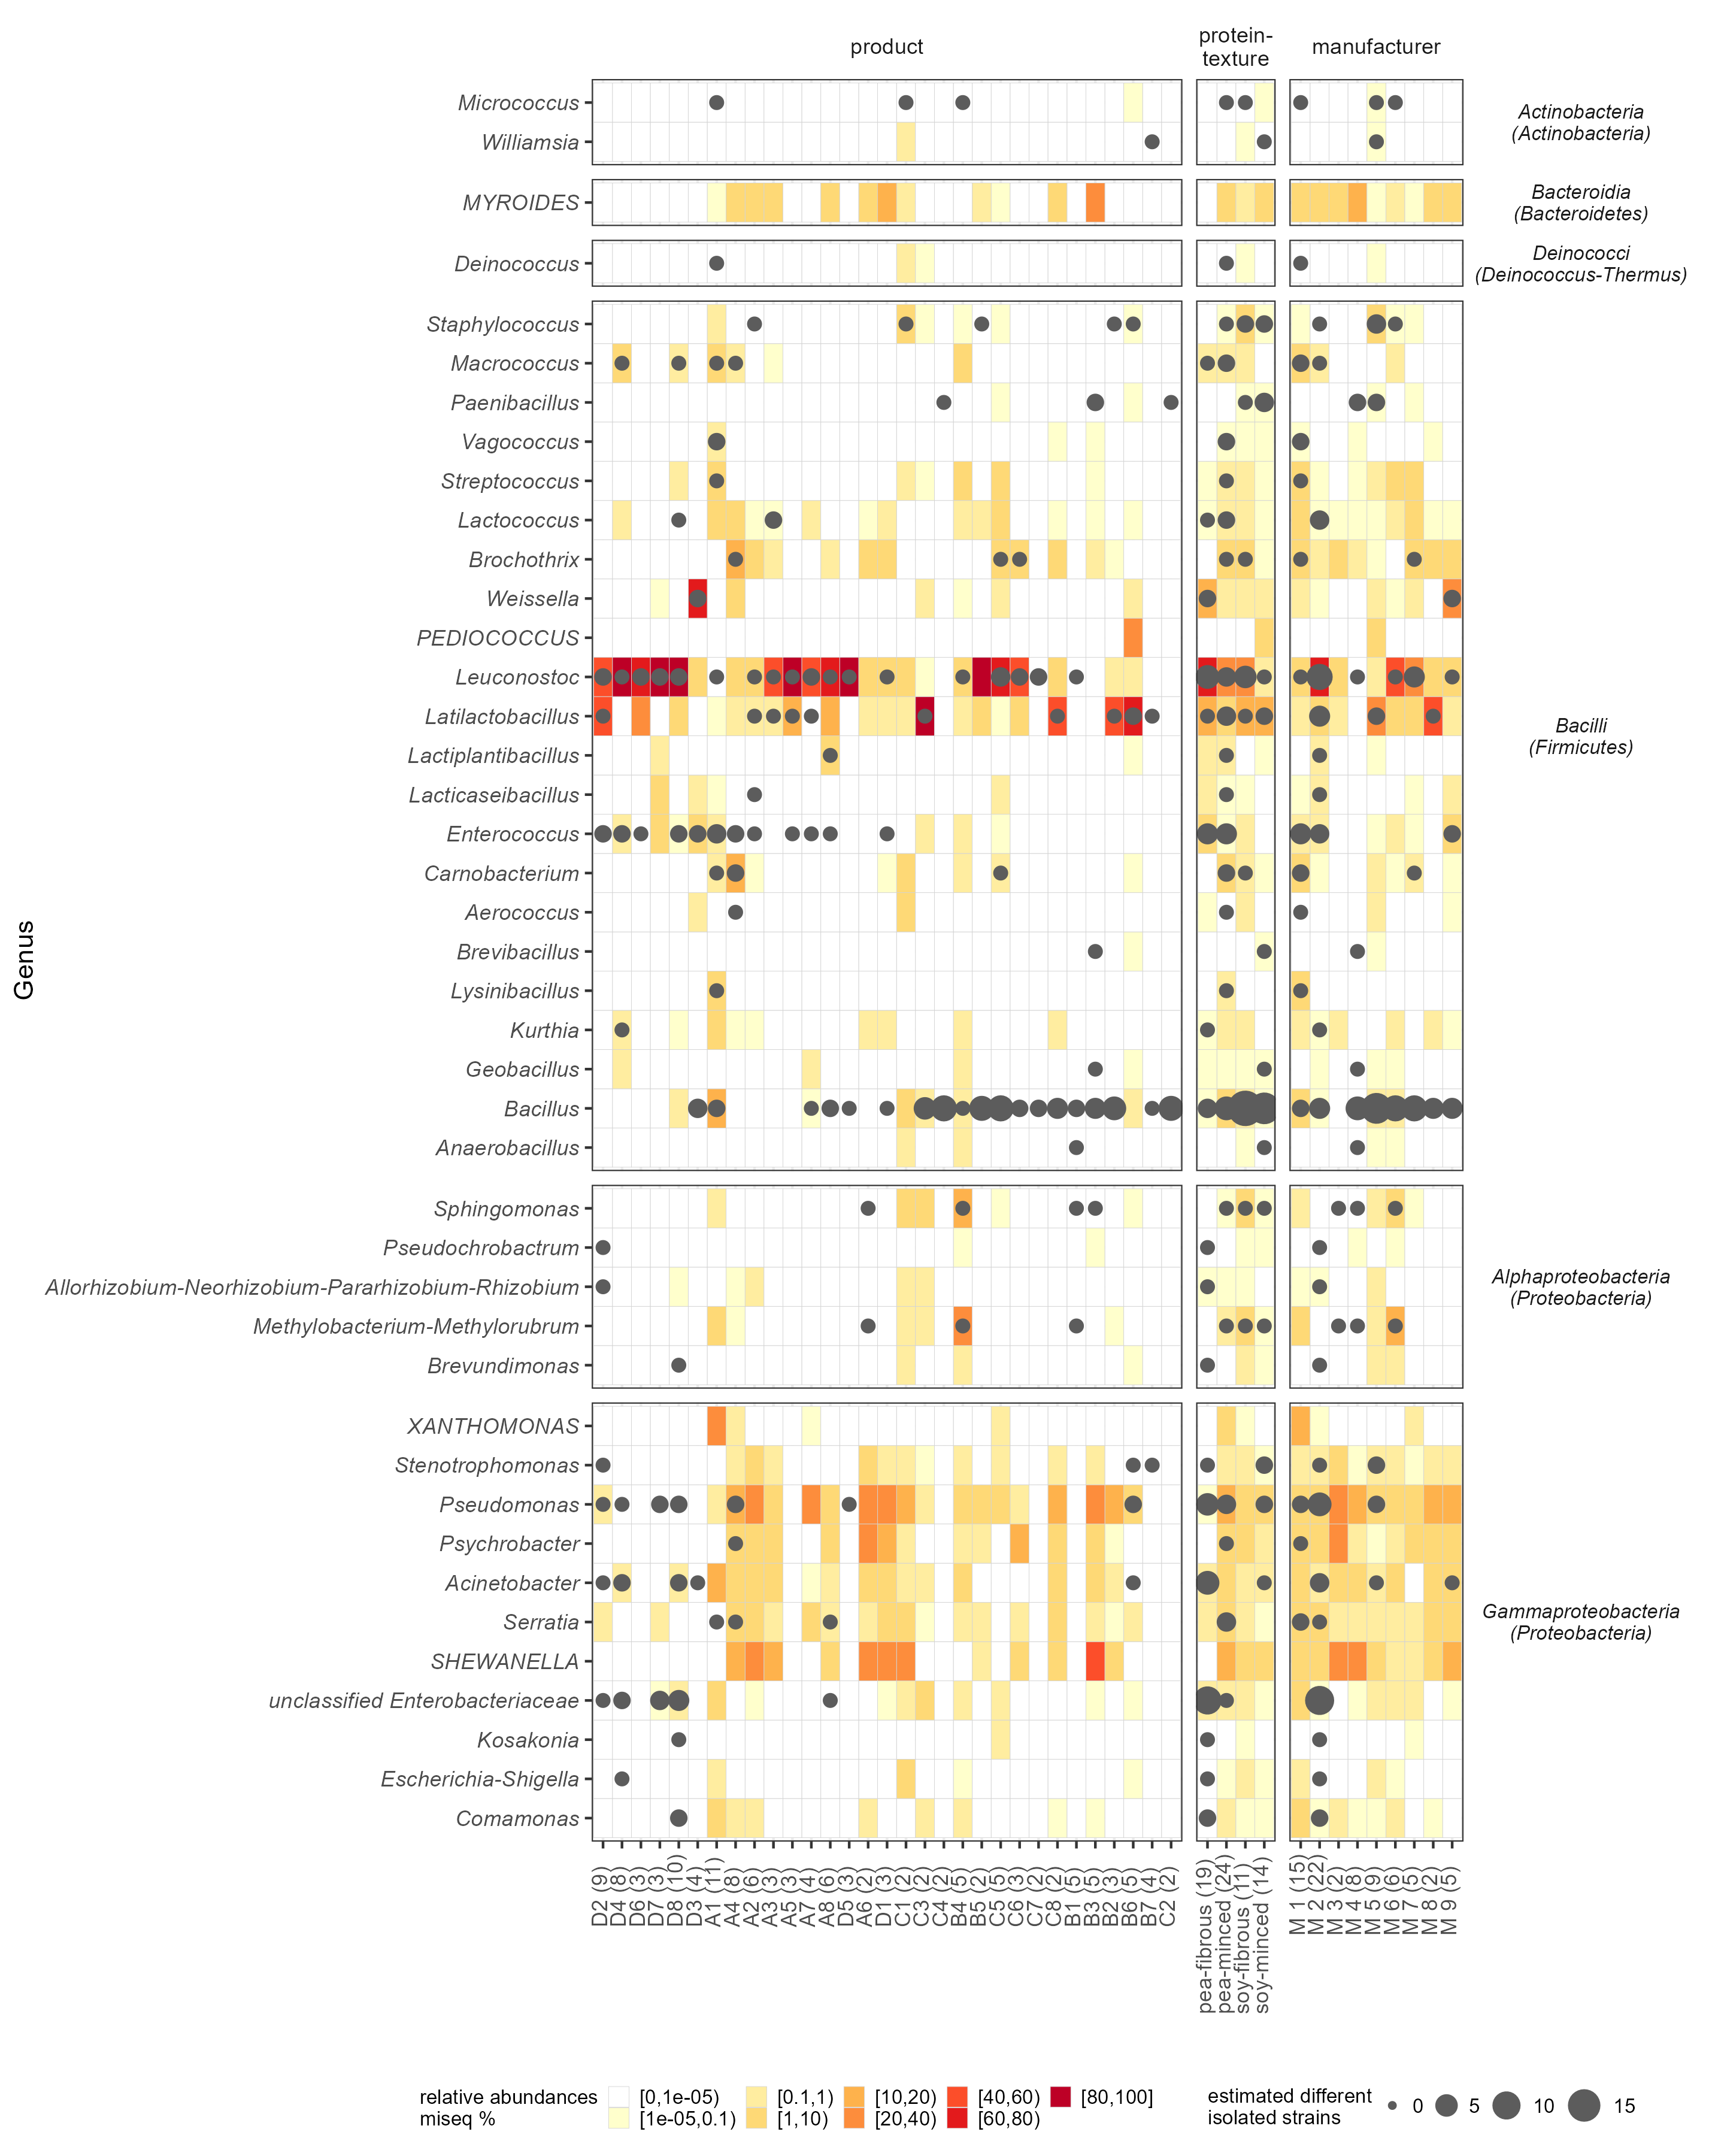
\includegraphics[width=1\linewidth]{Fig1inclmeanrelab} 

}

\caption{\label{fig1} Present isolates per sample, group or manufacturer are represented by dots. Isolates with a genus were clustered based on their 16S rRNA gene sequences. Different clusters represents different strains or species. The higher the number of clusters within a genus, the larger the plotted dot in the figure. The surrounding area is shaded according to the relative abundances in the amplicon sequencing (for the group and manufacturer summary, the mean relative abundance of each included sample is used).}\label{fig:fig1}
\end{figure}

\begin{figure}

{\centering 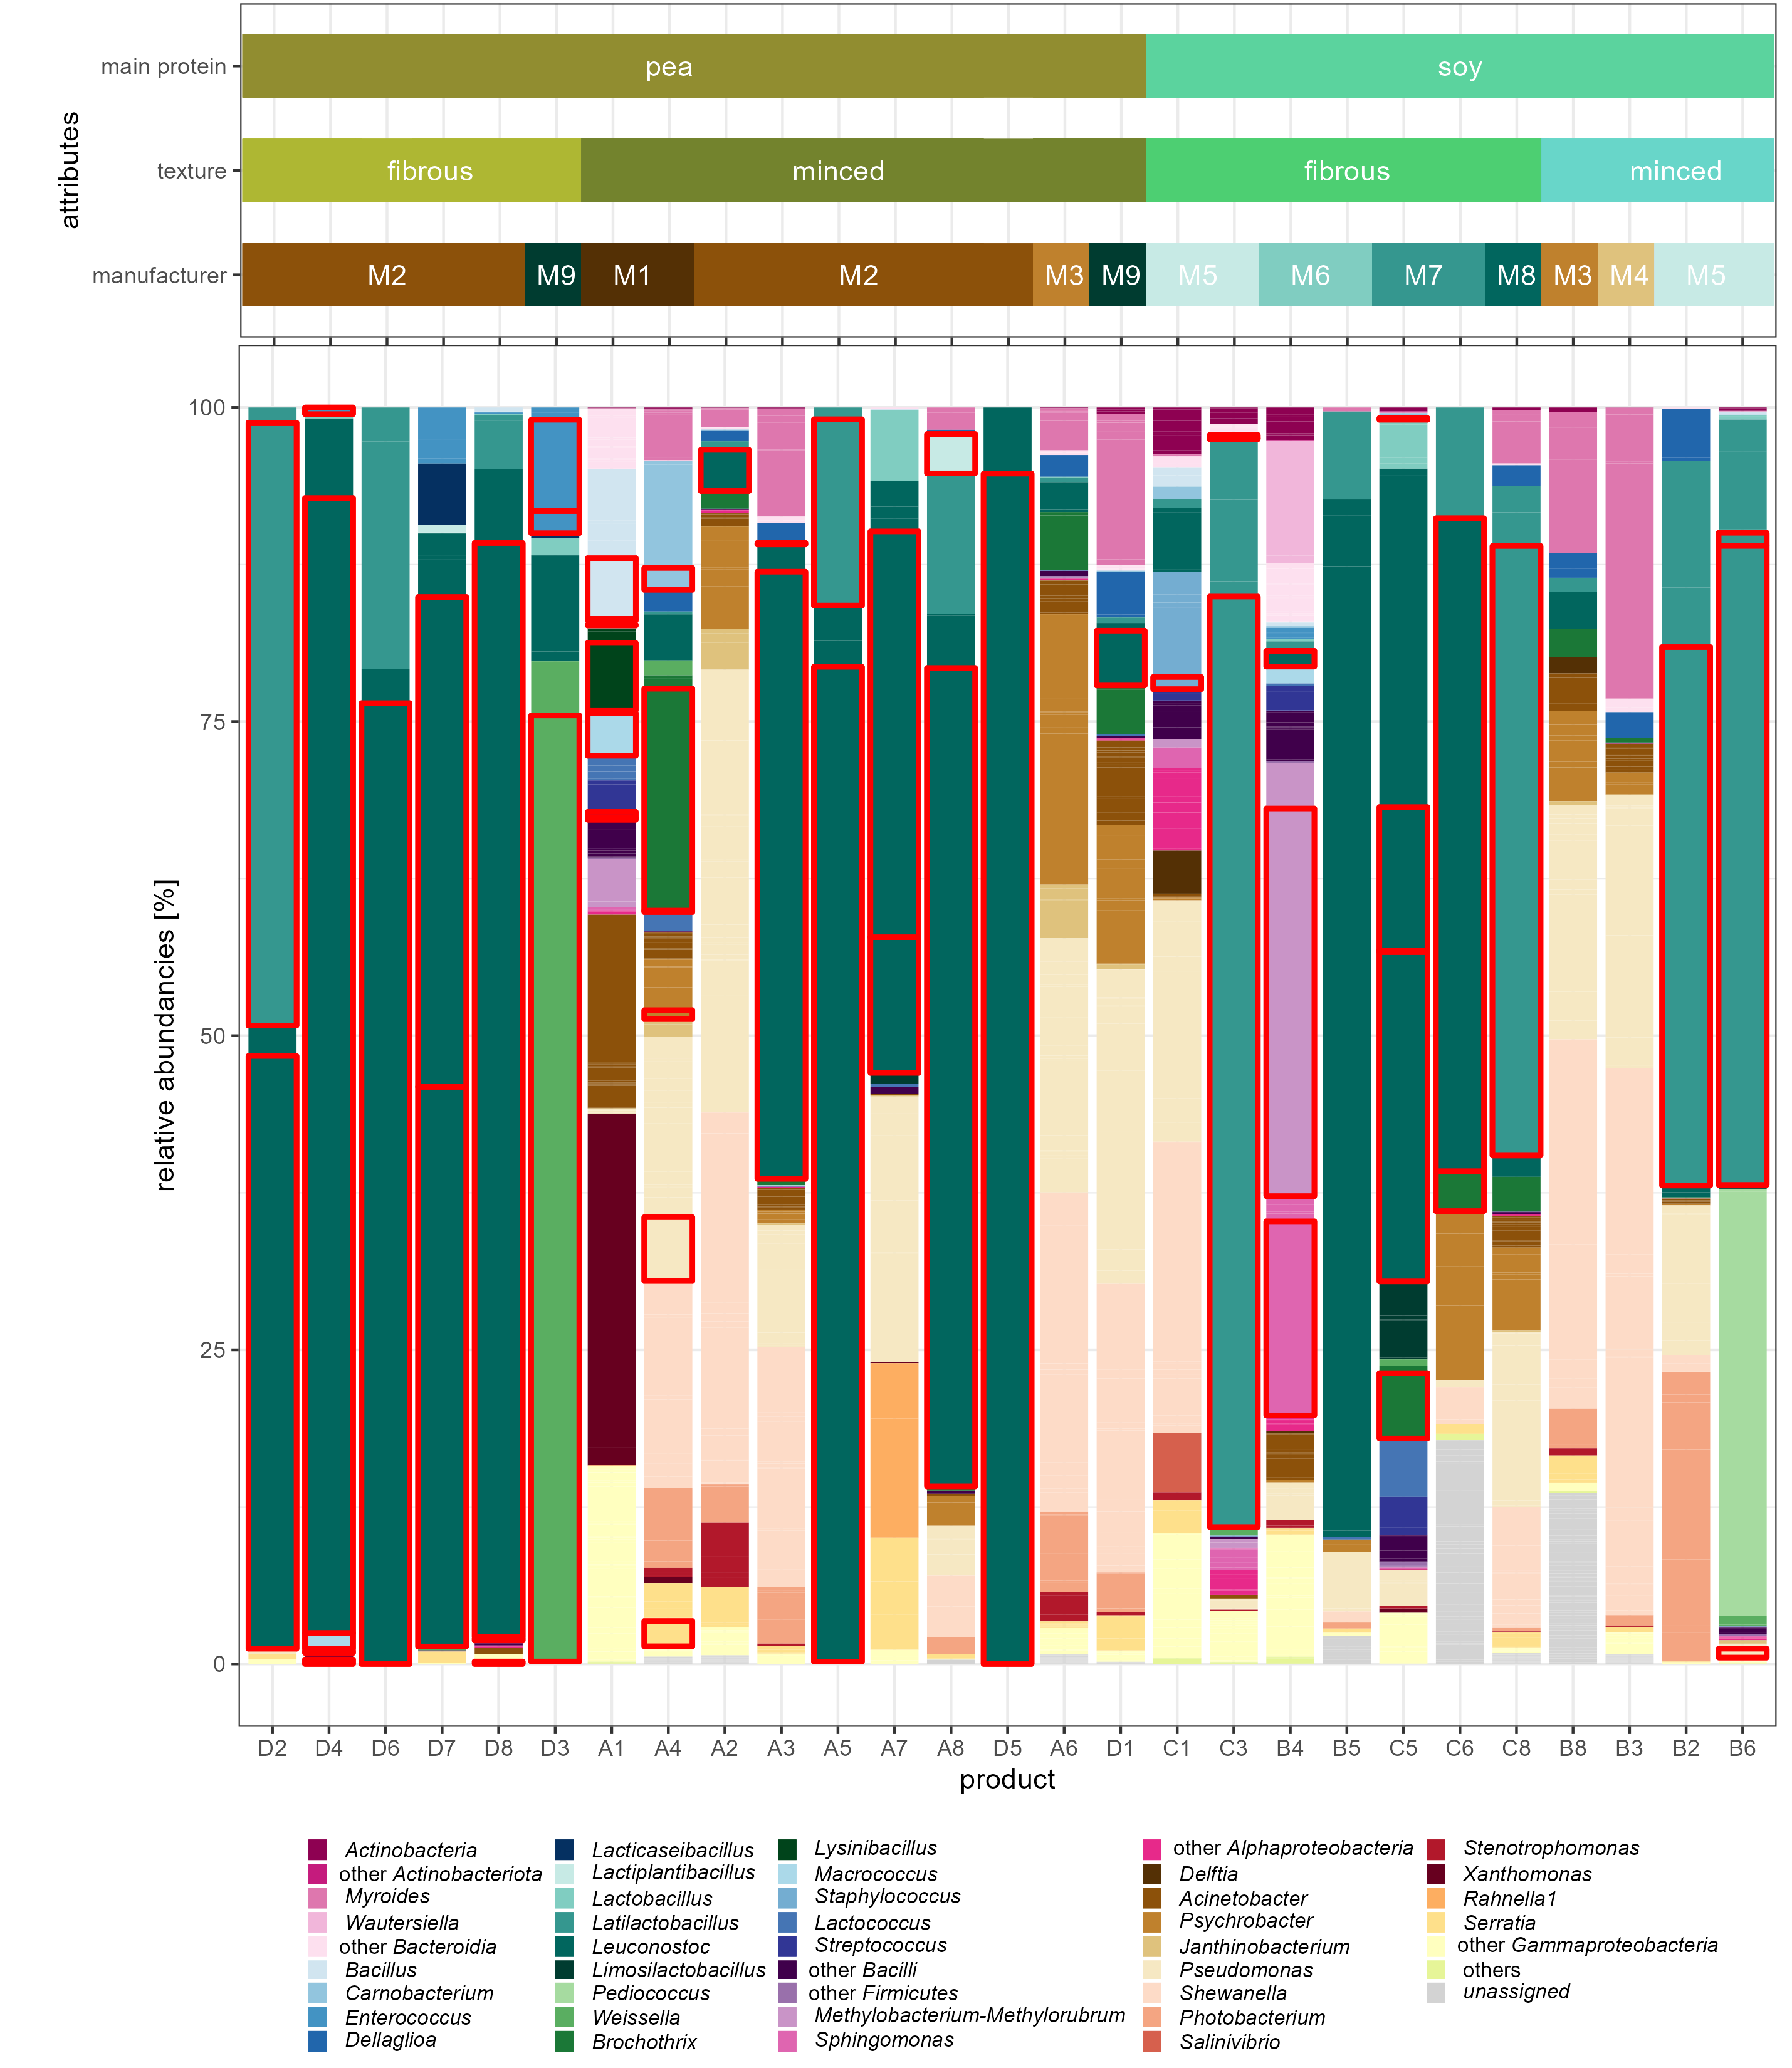
\includegraphics[width=1\linewidth]{Fig2_3percent} 

}

\caption{\label{fig2} Taxonomy plot based on amplicon sequencing, showing the relative abundances on genus level. The underlying relative frequencies of the ASVs are recognizable as pale yellow lines within a genus. Genera with a maximum value of 3\% across all samples were subsumed by color in the next higher taxonomic level.  The samples are ordered by main protein source, texture and manufacturer. ASVs with matching isolates (>99\% identity), were outlined in red.}\label{fig:fig2}
\end{figure}

\begin{figure}

{\centering 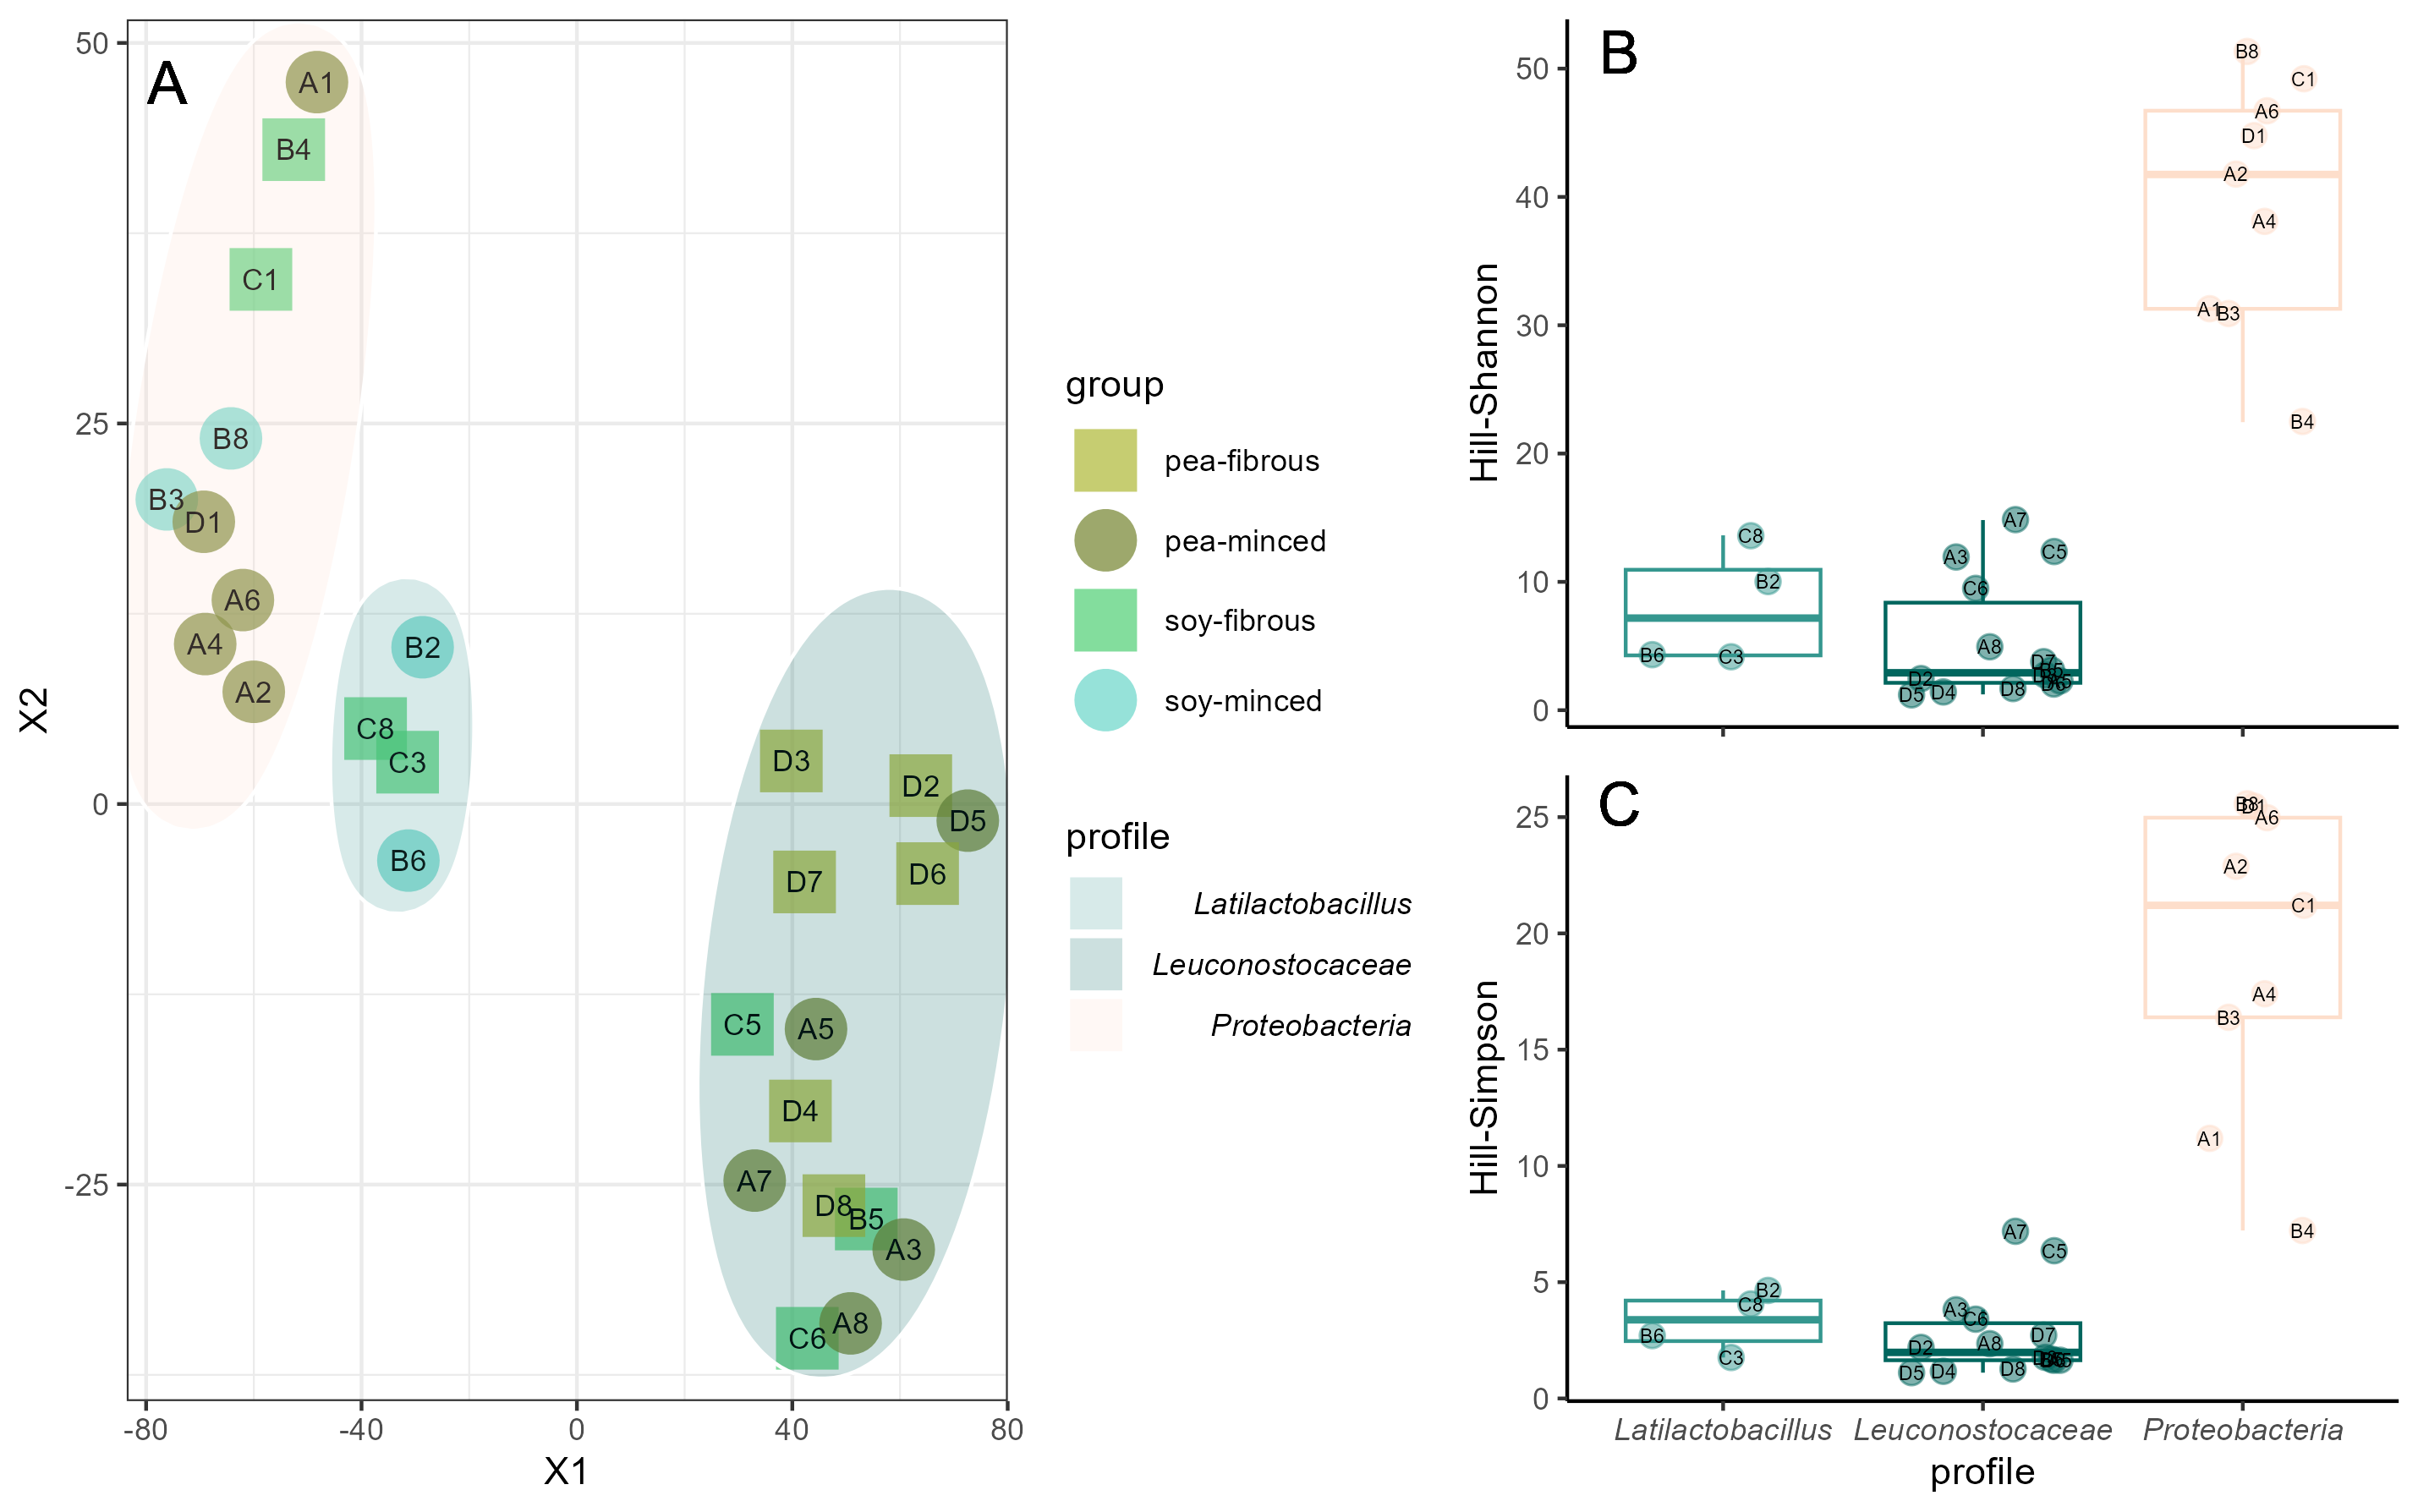
\includegraphics[width=1\linewidth]{Fig3profiles} 

}

\caption{\label{fig3} \textbf {A:} tSNE plot clustered samples to different profiles based on Bray-Curtis dissimilarity (Similar clusters were also found with other distance matrices - see Supplements \ref{figSM4}). \textbf {B:} Hill-Shannon diversity and \textbf {C:} Hill-Simpson diversity comparing these profiles. }\label{fig:fig3}
\end{figure}

\newpage

\hypertarget{supplementary-material}{%
\section*{Supplementary material}\label{supplementary-material}}
\addcontentsline{toc}{section}{Supplementary material}

\beginsupplement

\hypertarget{supplements}{%
\section{Supplements}\label{supplements}}

Supplement Table \ref{tabSM1}:

Supplement \ref{figSM1}: Groupwise comparison of the alpha-diversity
using Hill-Shannon and Hill-Simpson indices. Hill-Shannon index differed
significantly between fibrous and minced pea products (p-val=0.016).

Supplement \ref{figSM2}: NMDS plots using different distance methods.

Supplement \ref{figSM3}: tSNE plots based on Bray-Curtis dissimilarity,
Jaccard distance and Jensen-Shannon divergence. In all three methods,
the same clusters form.

Supplement \ref{figSM4}: LEfSe per group

Supplement \ref{figSM5}: LEfSe per profile.

\singlespacing

\begin{longtable}[b]{llllll}
\caption{\label{tab:tabSM1}\label{tabSM1}PERMANOVA results based on different distance matrices.}\\
\toprule
 & Df & Sum of Sqs & R2 & F & Pr. F\\
\midrule
\endfirsthead
\caption[]{\label{tabSM1}PERMANOVA results based on different distance matrices. \textit{(continued)}}\\
\toprule
 & Df & Sum of Sqs & R2 & F & Pr. F\\
\midrule
\endhead

\endfoot
\bottomrule
\endlastfoot
\addlinespace[0.3em]
\multicolumn{6}{l}{\textbf{Bray-Curtis}}\\
\addlinespace[0.3em]
\multicolumn{6}{l}{\textit{\makecell[l]{Permutation test for adonis under reduced model\\Terms added sequentially (first to last)\\Permutation: free\\Number of permutations: 999\\adonis2(formula = dmlistshort[[i]] \textasciitilde{} protein.source * texture,\\data = data.frame(sample\_data(relab\_po)), permutations = 999)}}}\\
\hspace{1em}\hspace{1em}protein source & 1 & 0.7258 & 0.0743 & 2.090 & 0.030\\
\hspace{1em}\hspace{1em}texture & 1 & 0.8391 & 0.0859 & 2.416 & 0.017\\
\hspace{1em}\hspace{1em}protein source:texture & 1 & 0.2185 & 0.0224 & 0.629 & 0.825\\
\hspace{1em}\hspace{1em}residual & 23 & 7.9874 & 0.8175 &  \vphantom{1} & \\
\hspace{1em}\hspace{1em}total & 26 & 9.7708 & 1.0000 &  \vphantom{1} & \\
\addlinespace[0.3em]
\multicolumn{6}{l}{\textit{\makecell[l]{Permutation test for adonis under reduced model\\Terms added sequentially (first to last)\\Permutation: free\\Number of permutations: 999\\adonis2(formula = dmlistshort[[i]] \textasciitilde{} texture * protein.source,\\data = data.frame(sample\_data(relab\_po)), permutations = 999)}}}\\
\hspace{1em}\hspace{1em}protein source & 1 & 0.6784 & 0.0694 & 1.953 & 0.041\\
\hspace{1em}\hspace{1em}texture & 1 & 0.8864 & 0.0907 & 2.553 & 0.017\\
\hspace{1em}\hspace{1em}protein source:texture & 1 & 0.2185 & 0.0224 & 0.629 & 0.834\\
\hspace{1em}\hspace{1em}residual & 23 & 7.9874 & 0.8175 &  & \\
\hspace{1em}\hspace{1em}total & 26 & 9.7708 & 1.0000 &  & \\
\addlinespace[0.3em]
\multicolumn{6}{l}{\textbf{Jaccard}}\\
\addlinespace[0.3em]
\multicolumn{6}{l}{\textit{\makecell[l]{Permutation test for adonis under reduced model\\Terms added sequentially (first to last)\\Permutation: free\\Number of permutations: 999\\adonis2(formula = dmlistshort[[i]] \textasciitilde{} protein.source * texture,\\data = data.frame(sample\_data(relab\_po)), permutations = 999)}}}\\
\hspace{1em}\hspace{1em}protein source & 1 & 0.6774 & 0.0626 & 1.712 & 0.041\\
\hspace{1em}\hspace{1em}texture & 1 & 0.7484 & 0.0691 & 1.891 & 0.022\\
\hspace{1em}\hspace{1em}protein source:texture & 1 & 0.3001 & 0.0277 & 0.758 & 0.789\\
\hspace{1em}\hspace{1em}residual & 23 & 9.1035 & 0.8406 &  \vphantom{1} & \\
\hspace{1em}\hspace{1em}total & 26 & 10.8295 & 1.0000 &  \vphantom{1} & \\
\addlinespace[0.3em]
\multicolumn{6}{l}{\textit{\makecell[l]{Permutation test for adonis under reduced model\\Terms added sequentially (first to last)\\Permutation: free\\Number of permutations: 999\\adonis2(formula = dmlistshort[[i]] \textasciitilde{} texture * protein.source,\\data = data.frame(sample\_data(relab\_po)), permutations = 999)}}}\\
\hspace{1em}\hspace{1em}protein source & 1 & 0.6367 & 0.0588 & 1.609 & 0.065\\
\hspace{1em}\hspace{1em}texture & 1 & 0.7891 & 0.0729 & 1.994 & 0.014\\
\hspace{1em}\hspace{1em}protein source:texture & 1 & 0.3001 & 0.0277 & 0.758 & 0.770\\
\hspace{1em}\hspace{1em}residual & 23 & 9.1035 & 0.8406 &  & \\
\hspace{1em}\hspace{1em}total & 26 & 10.8295 & 1.0000 &  & \\
\addlinespace[0.3em]
\multicolumn{6}{l}{\textbf{Jensen-Shannon}}\\
\addlinespace[0.3em]
\multicolumn{6}{l}{\textit{\makecell[l]{Permutation test for adonis under reduced model\\Terms added sequentially (first to last)\\Permutation: free\\Number of permutations: 999\\adonis2(formula = dmlistshort[[i]] \textasciitilde{} protein.source * texture,\\data = data.frame(sample\_data(relab\_po)), permutations = 999)}}}\\
\hspace{1em}\hspace{1em}protein source & 1 & 0.3254 & 0.0874 & 2.626 & 0.034\\
\hspace{1em}\hspace{1em}texture & 1 & 0.4556 & 0.1224 & 3.676 & 0.008\\
\hspace{1em}\hspace{1em}protein source:texture & 1 & 0.0918 & 0.0246 & 0.740 & 0.607\\
\hspace{1em}\hspace{1em}residual & 23 & 2.8504 & 0.7656 &  \vphantom{1} & \\
\hspace{1em}\hspace{1em}total & 26 & 3.7231 & 1.0000 &  \vphantom{1} & \\
\addlinespace[0.3em]
\multicolumn{6}{l}{\textit{\makecell[l]{Permutation test for adonis under reduced model\\Terms added sequentially (first to last)\\Permutation: free\\Number of permutations: 999\\adonis2(formula = dmlistshort[[i]] \textasciitilde{} texture * protein.source,\\data = data.frame(sample\_data(relab\_po)), permutations = 999)}}}\\
\hspace{1em}\hspace{1em}protein source & 1 & 0.3698 & 0.0993 & 2.984 & 0.019\\
\hspace{1em}\hspace{1em}texture & 1 & 0.4111 & 0.1104 & 3.318 & 0.007\\
\hspace{1em}\hspace{1em}protein source:texture & 1 & 0.0918 & 0.0246 & 0.740 & 0.609\\
\hspace{1em}\hspace{1em}residual & 23 & 2.8504 & 0.7656 &  & \\
\hspace{1em}\hspace{1em}total & 26 & 3.7231 & 1.0000 &  & \\*
\end{longtable}

\doublespacing

\begin{figure}

{\centering 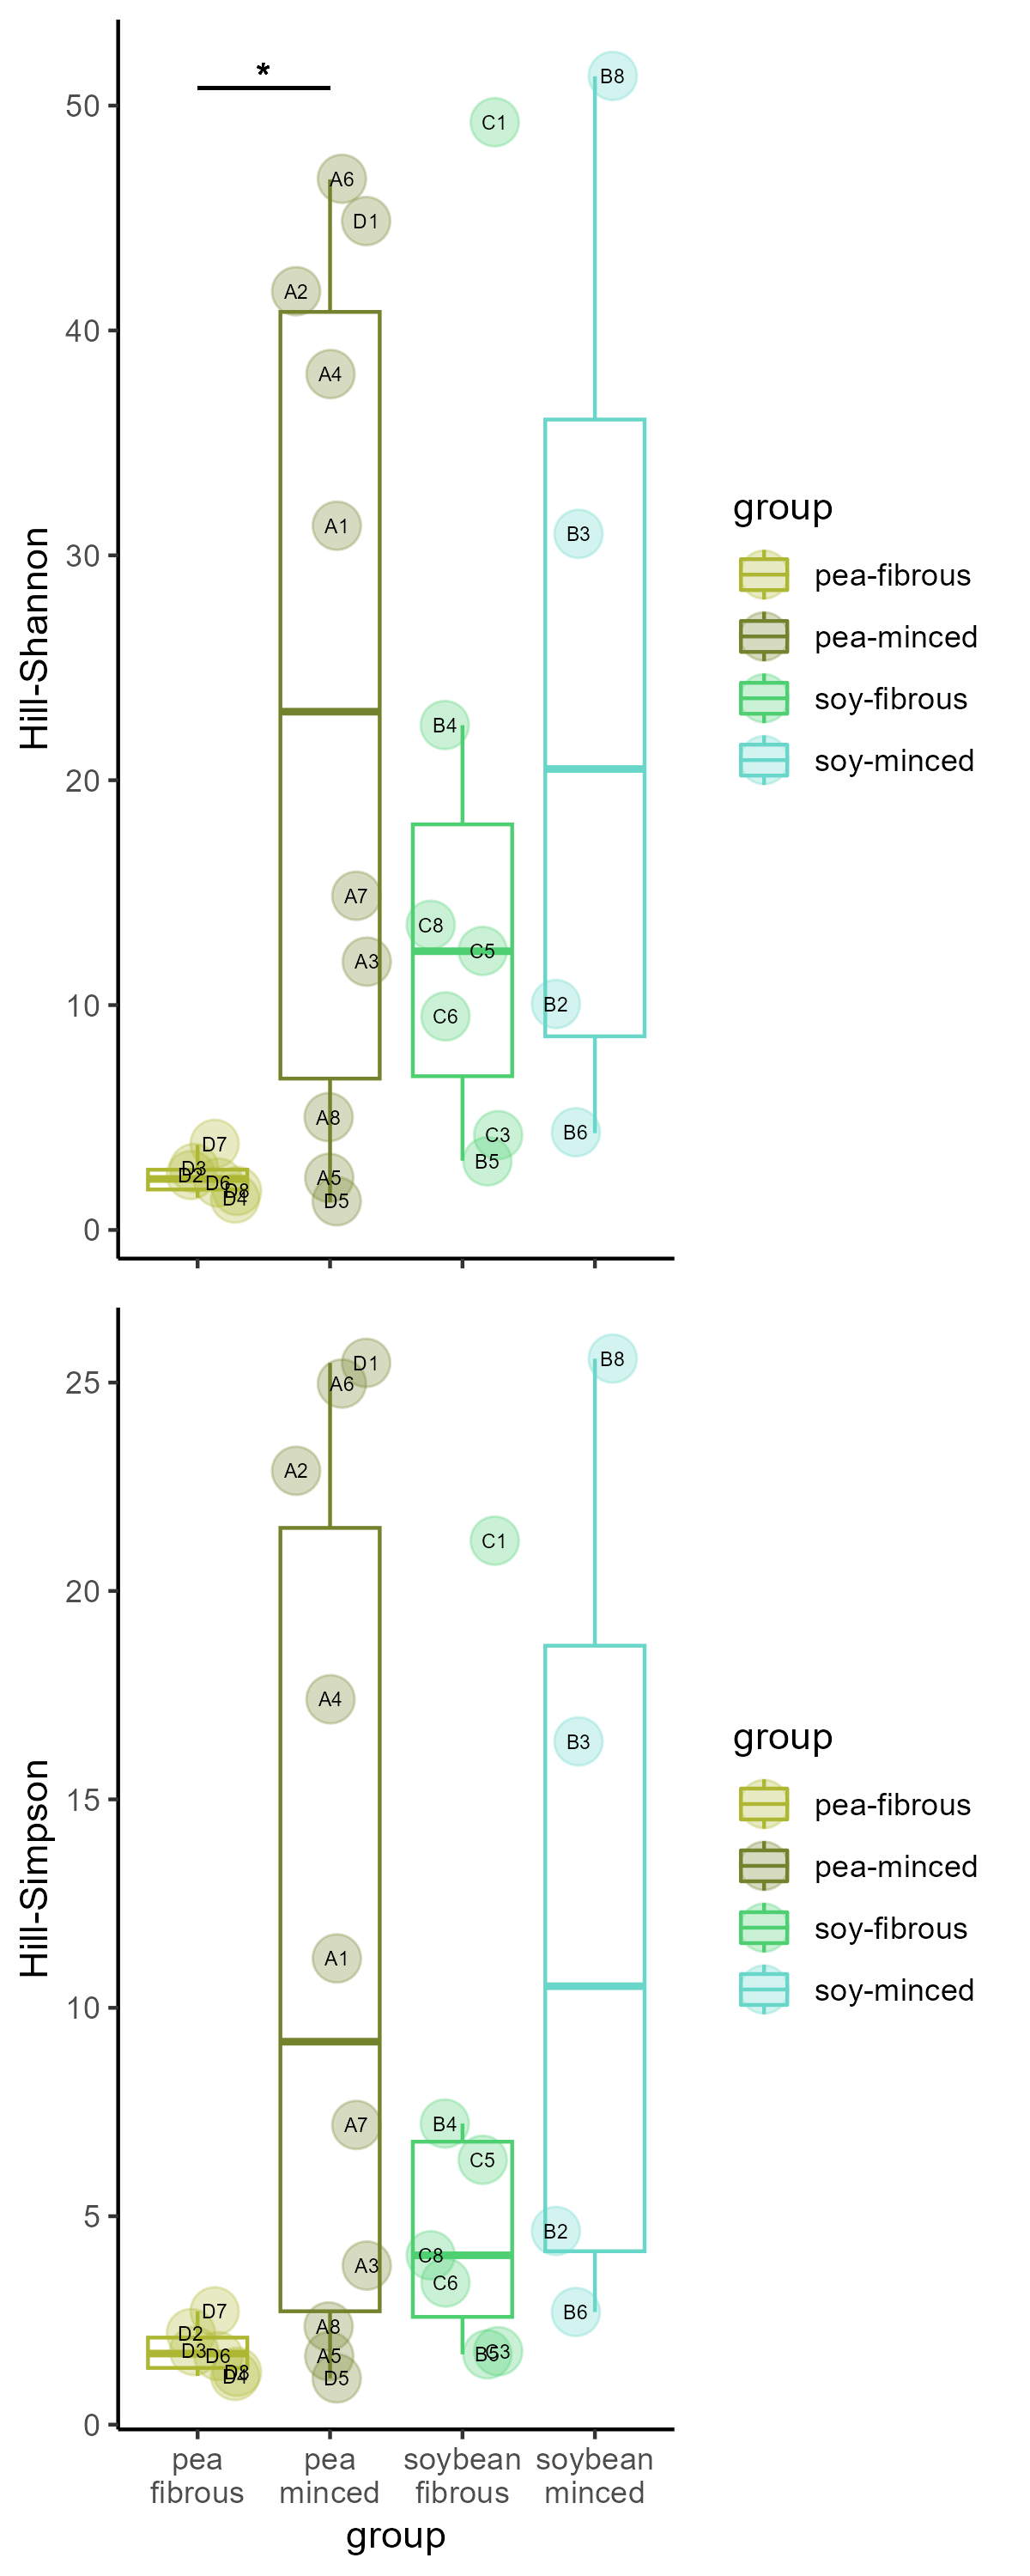
\includegraphics[width=0.5\linewidth]{PlotDivByCov} 

}

\caption{\label{figSM1} Groupwise comparison of the alpha-diversity using Hill-Shannon and Hill-Simpson indices. Hill-Shannon index differed significantly between fibrous and minced pea products (p-val=0.016).}\label{fig:figSM1}
\end{figure}

\begin{figure}

{\centering 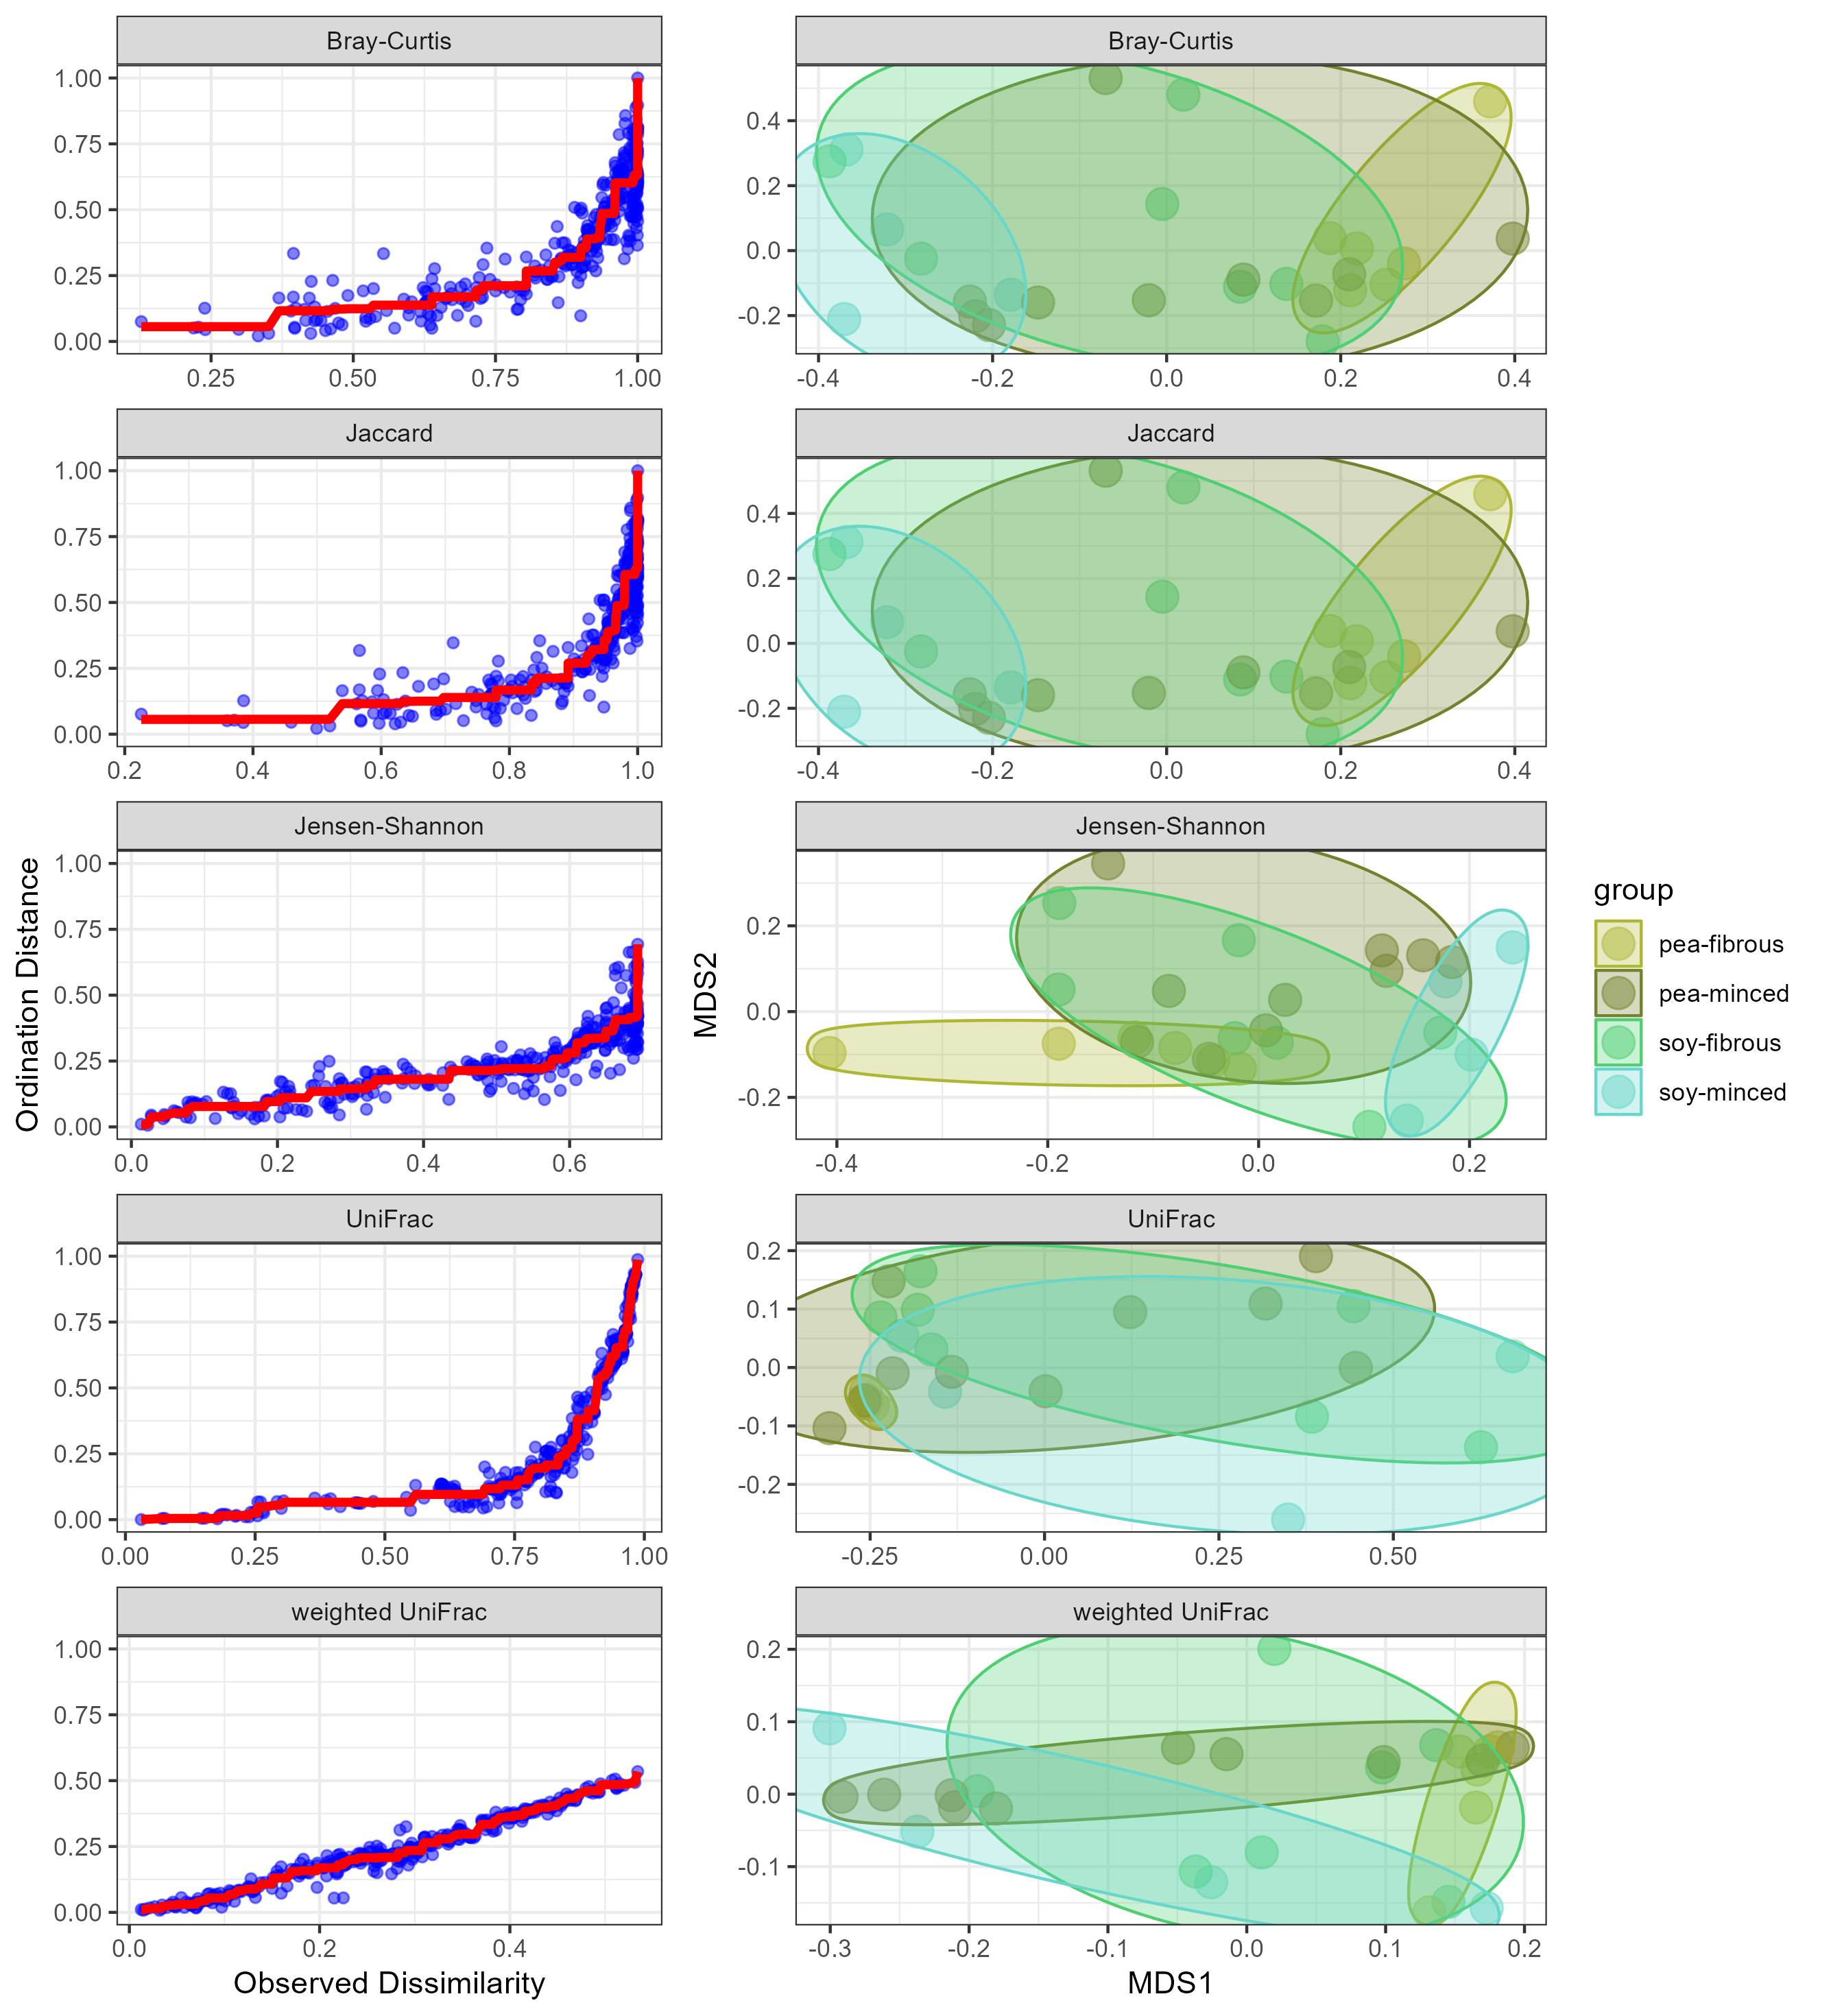
\includegraphics[width=1\linewidth]{NMDSplots} 

}

\caption{\label{figSM2} NMDS plots using different distance methods.  }\label{fig:figSM2}
\end{figure}

\begin{figure}

{\centering 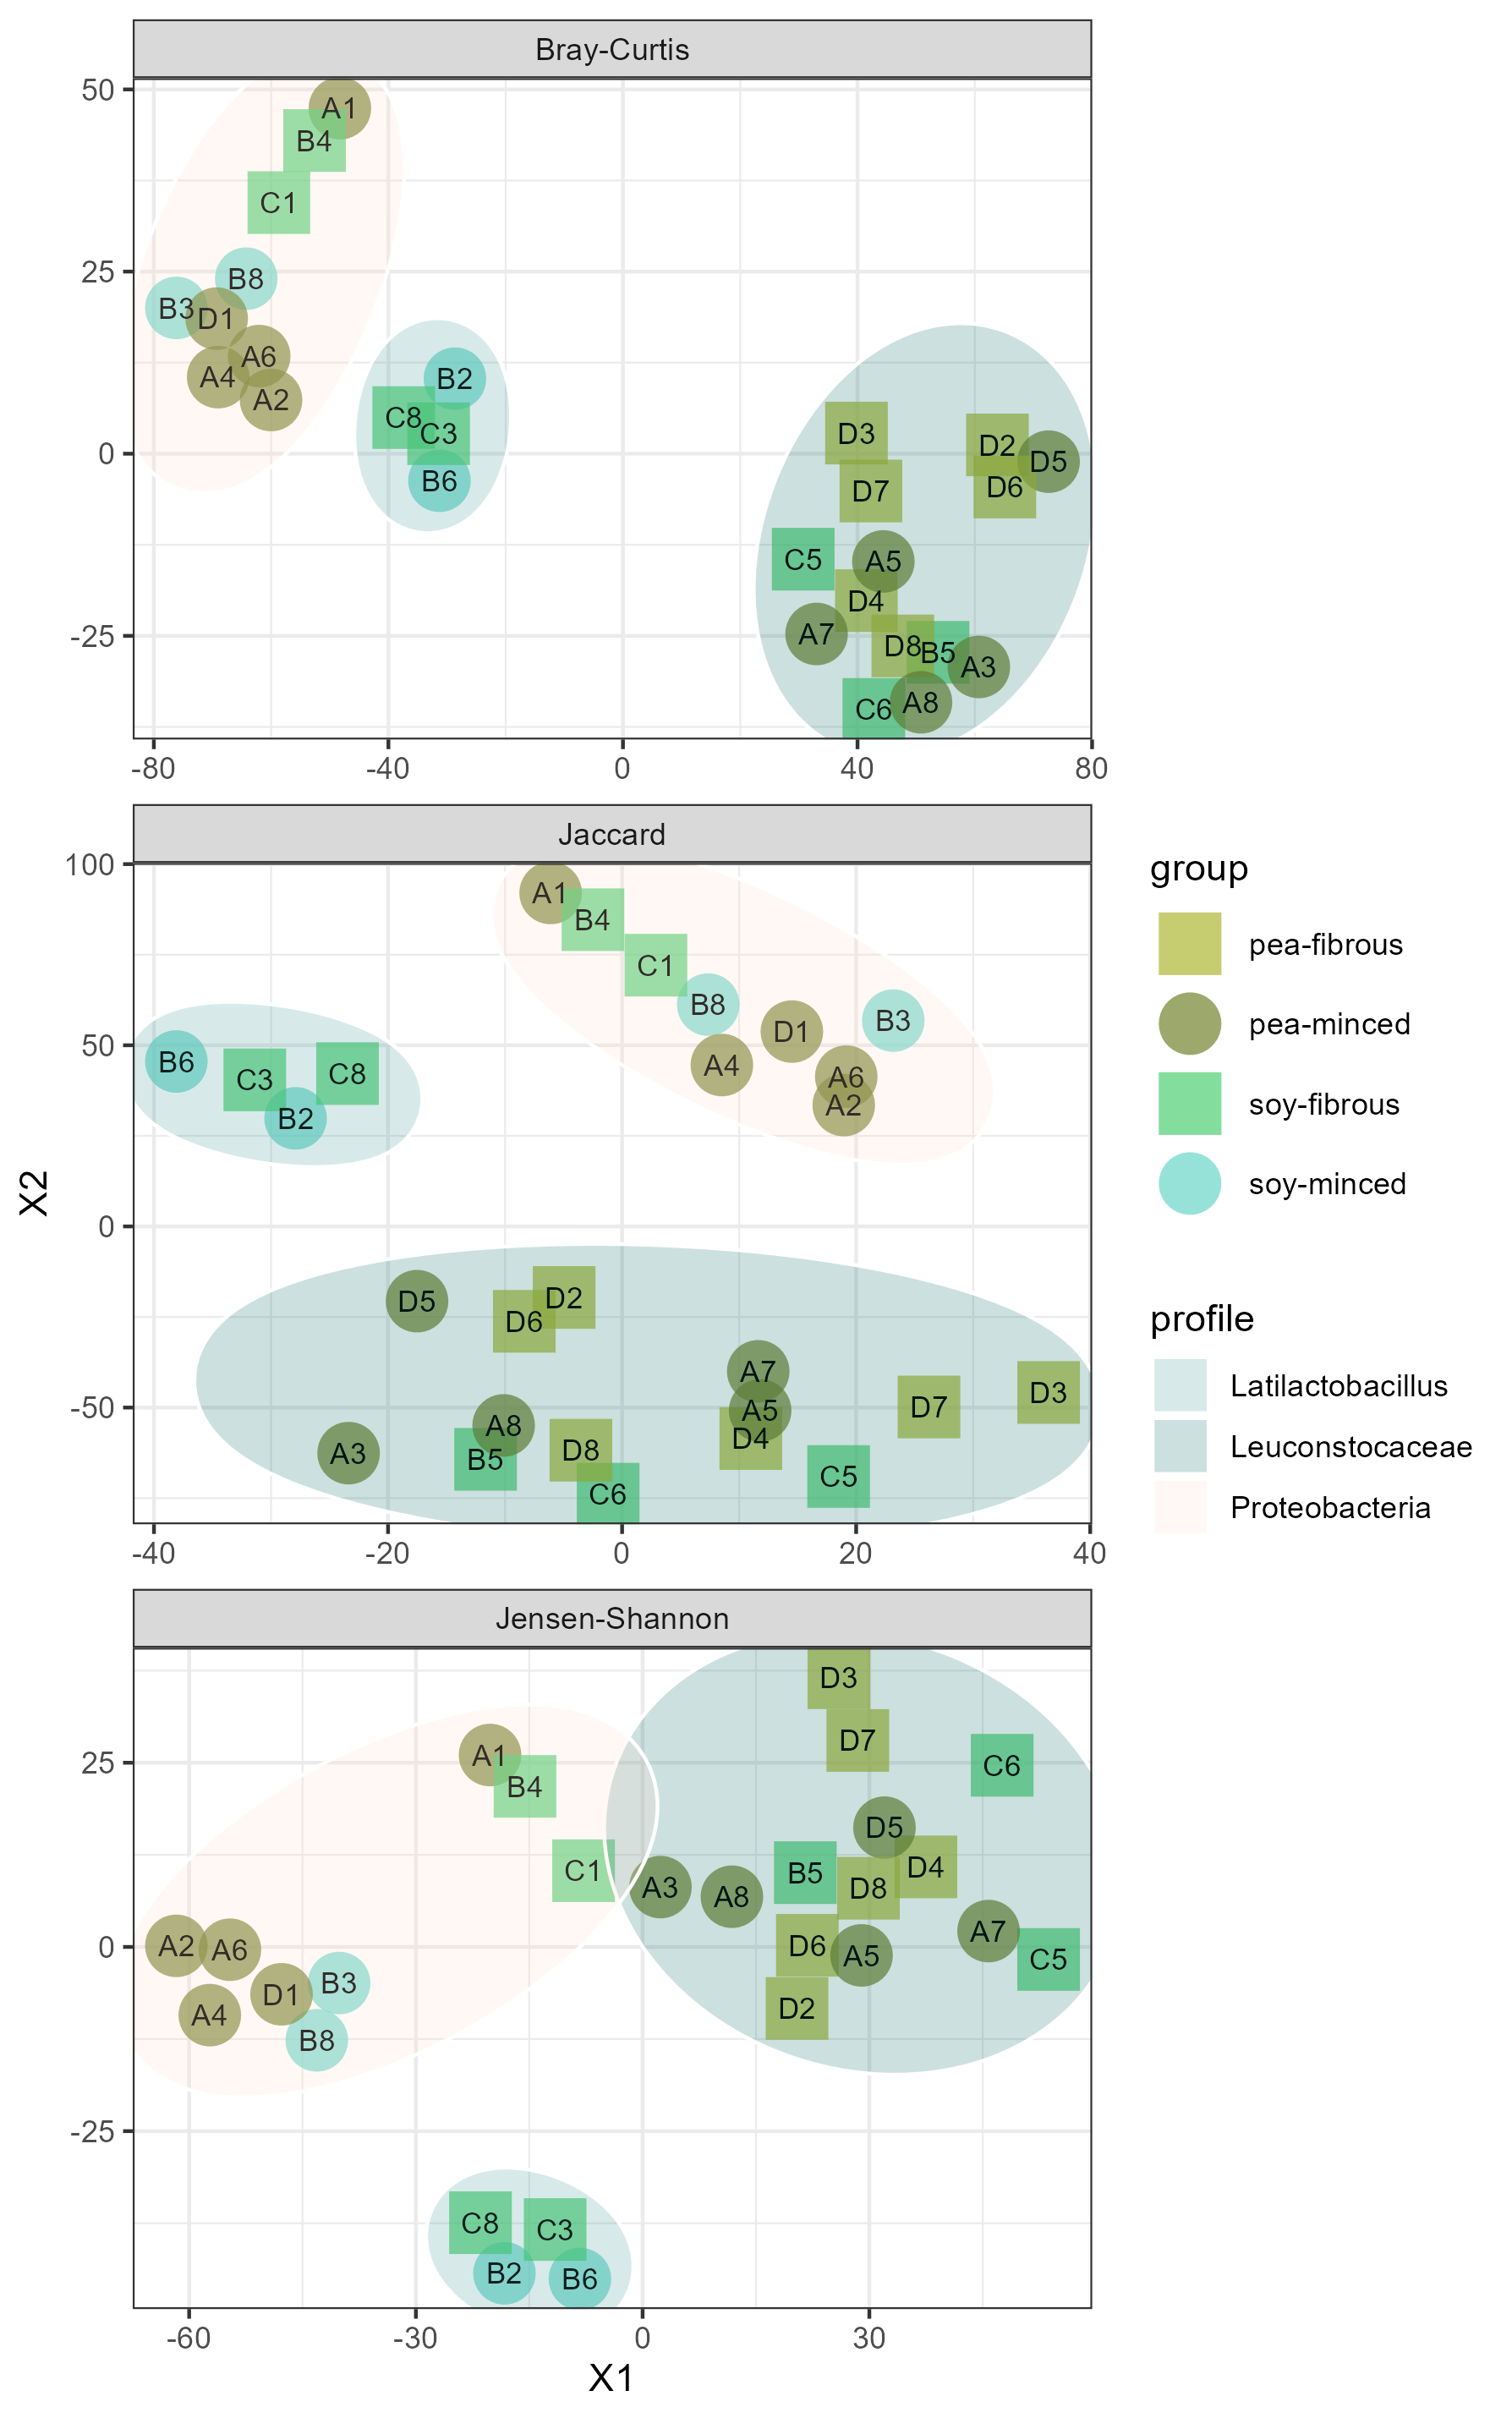
\includegraphics[width=0.8\linewidth]{FigSM4} 

}

\caption{\label{figSM3} tSNE plots based on Bray-Curtis dissimilarity, Jaccard distance and Jensen-Shannon divergence. In all three methods, the same clusters form.  }\label{fig:figSM3}
\end{figure}

\begin{figure}

{\centering 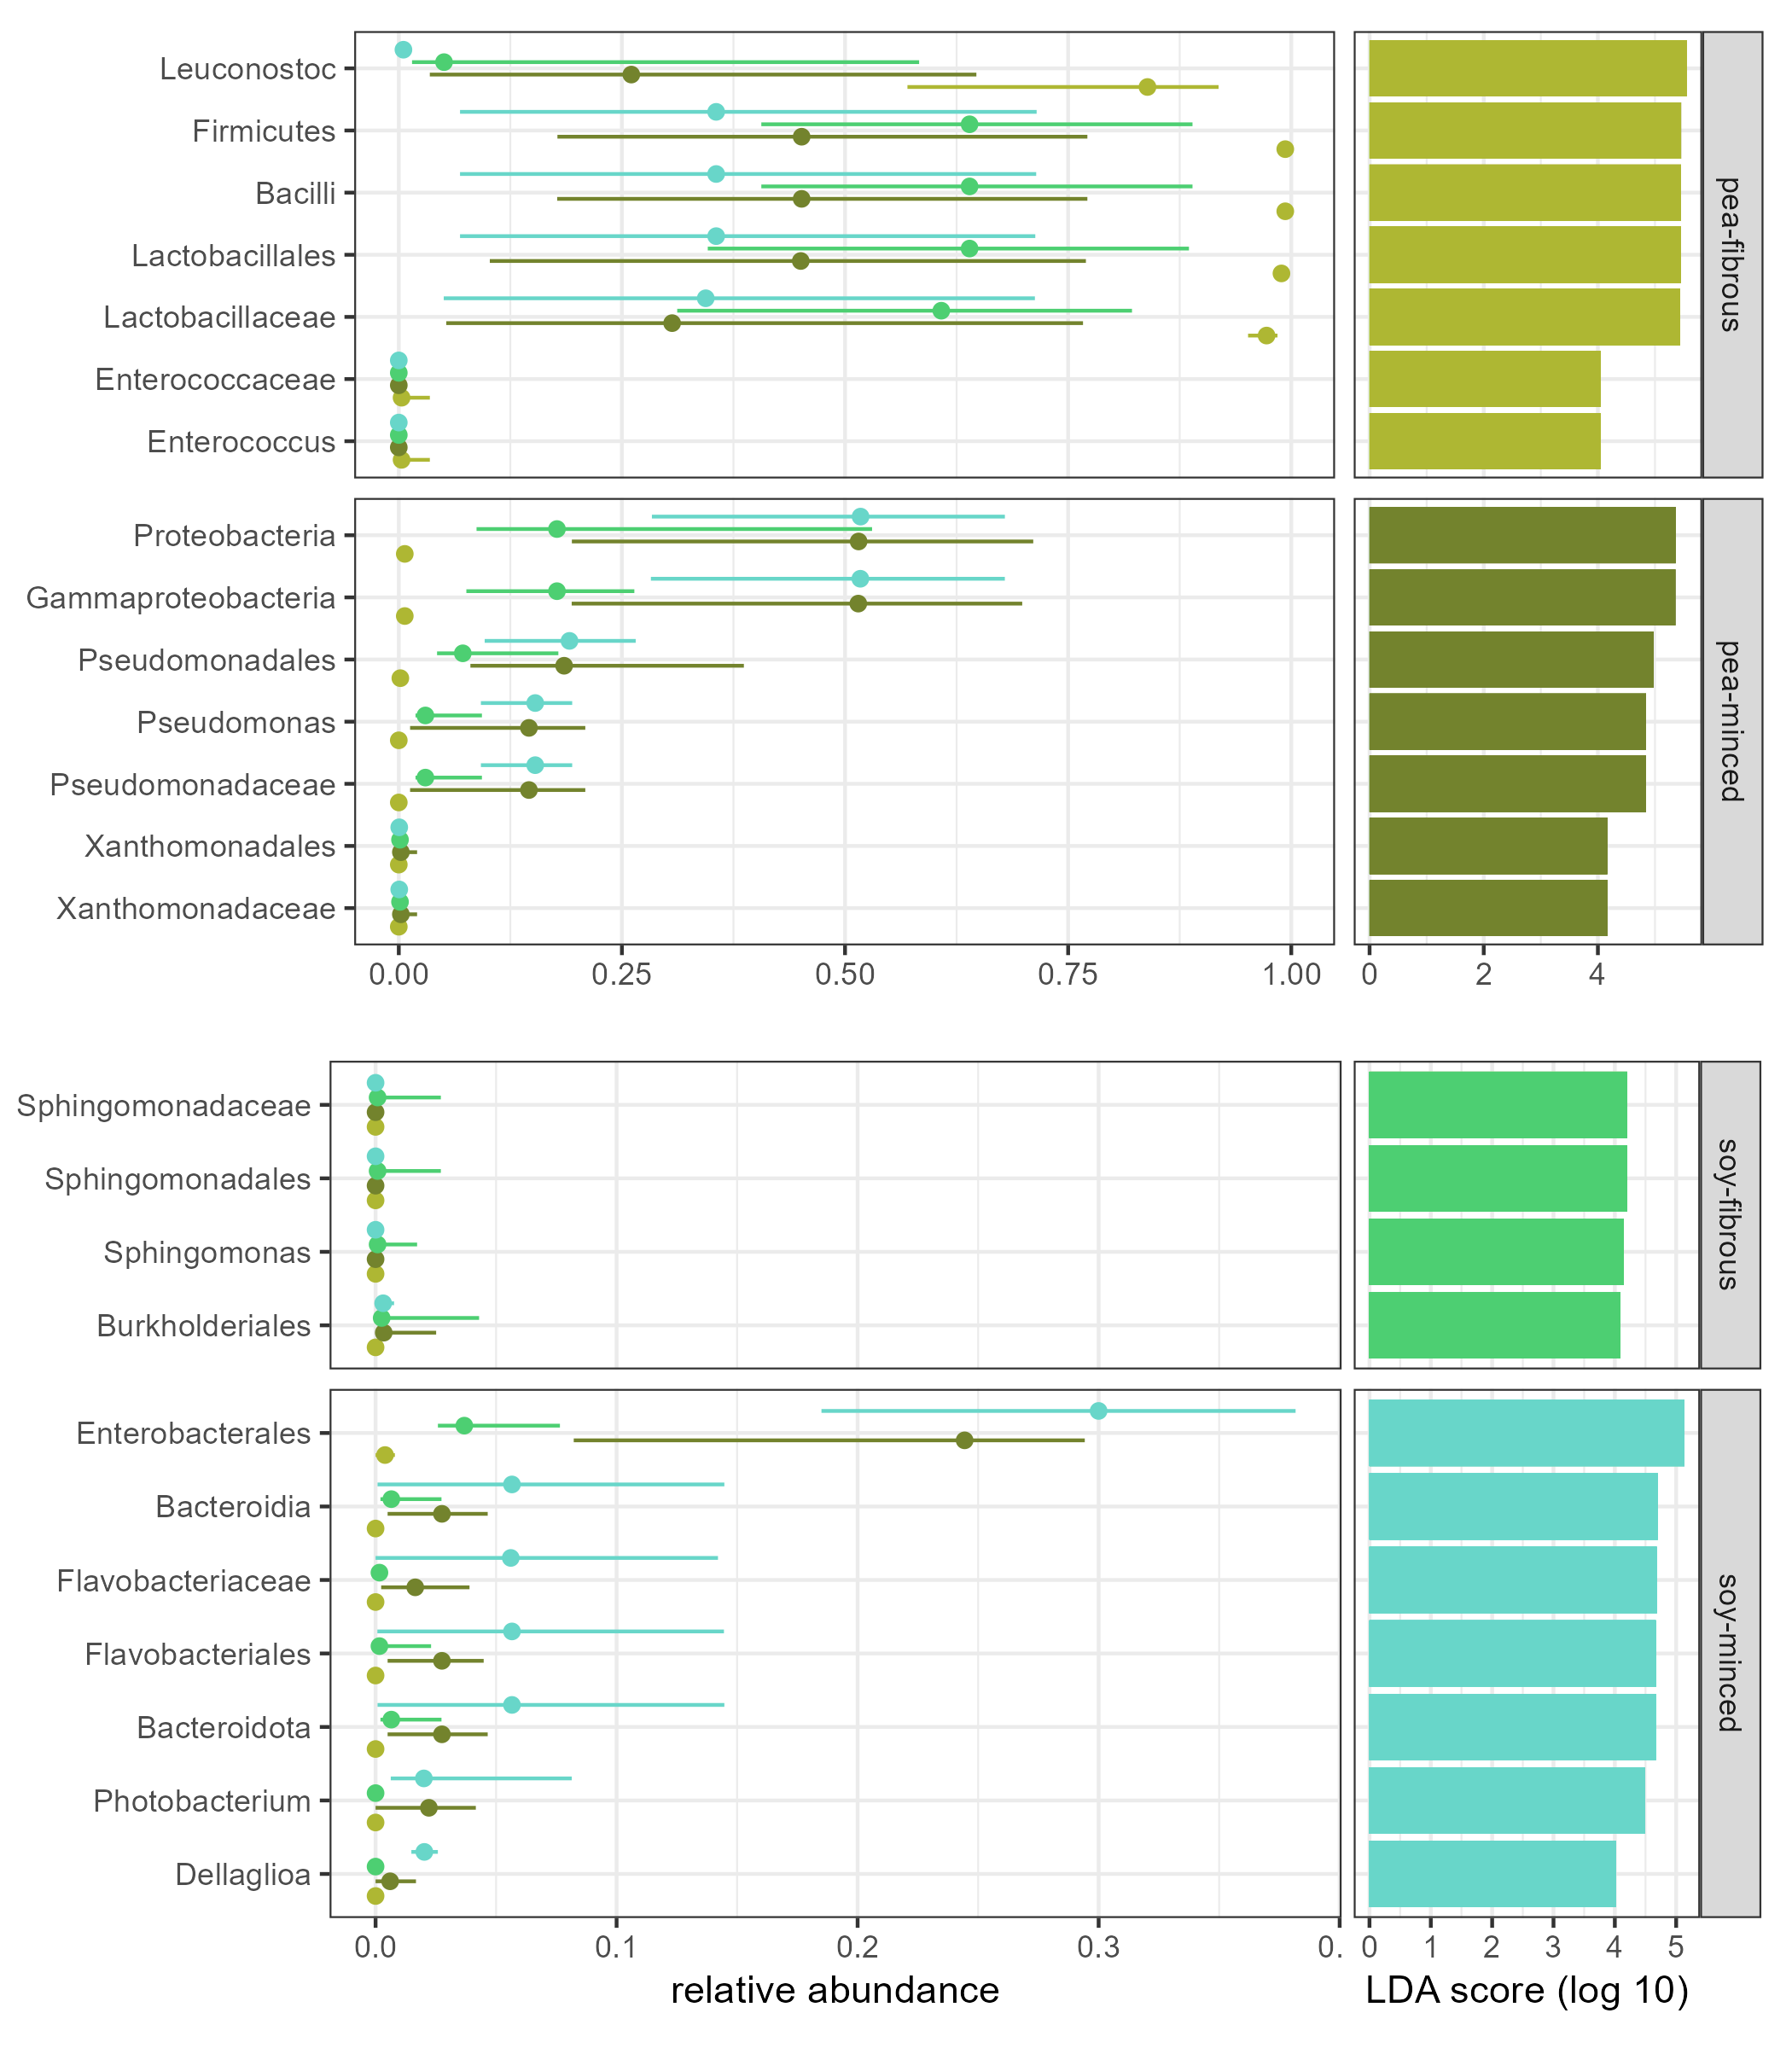
\includegraphics[width=1\linewidth]{lefsestatplotdiffscales} 

}

\caption{\label{figSM4} LEfSe per group.  }\label{fig:figSM4}
\end{figure}

\begin{figure}

{\centering 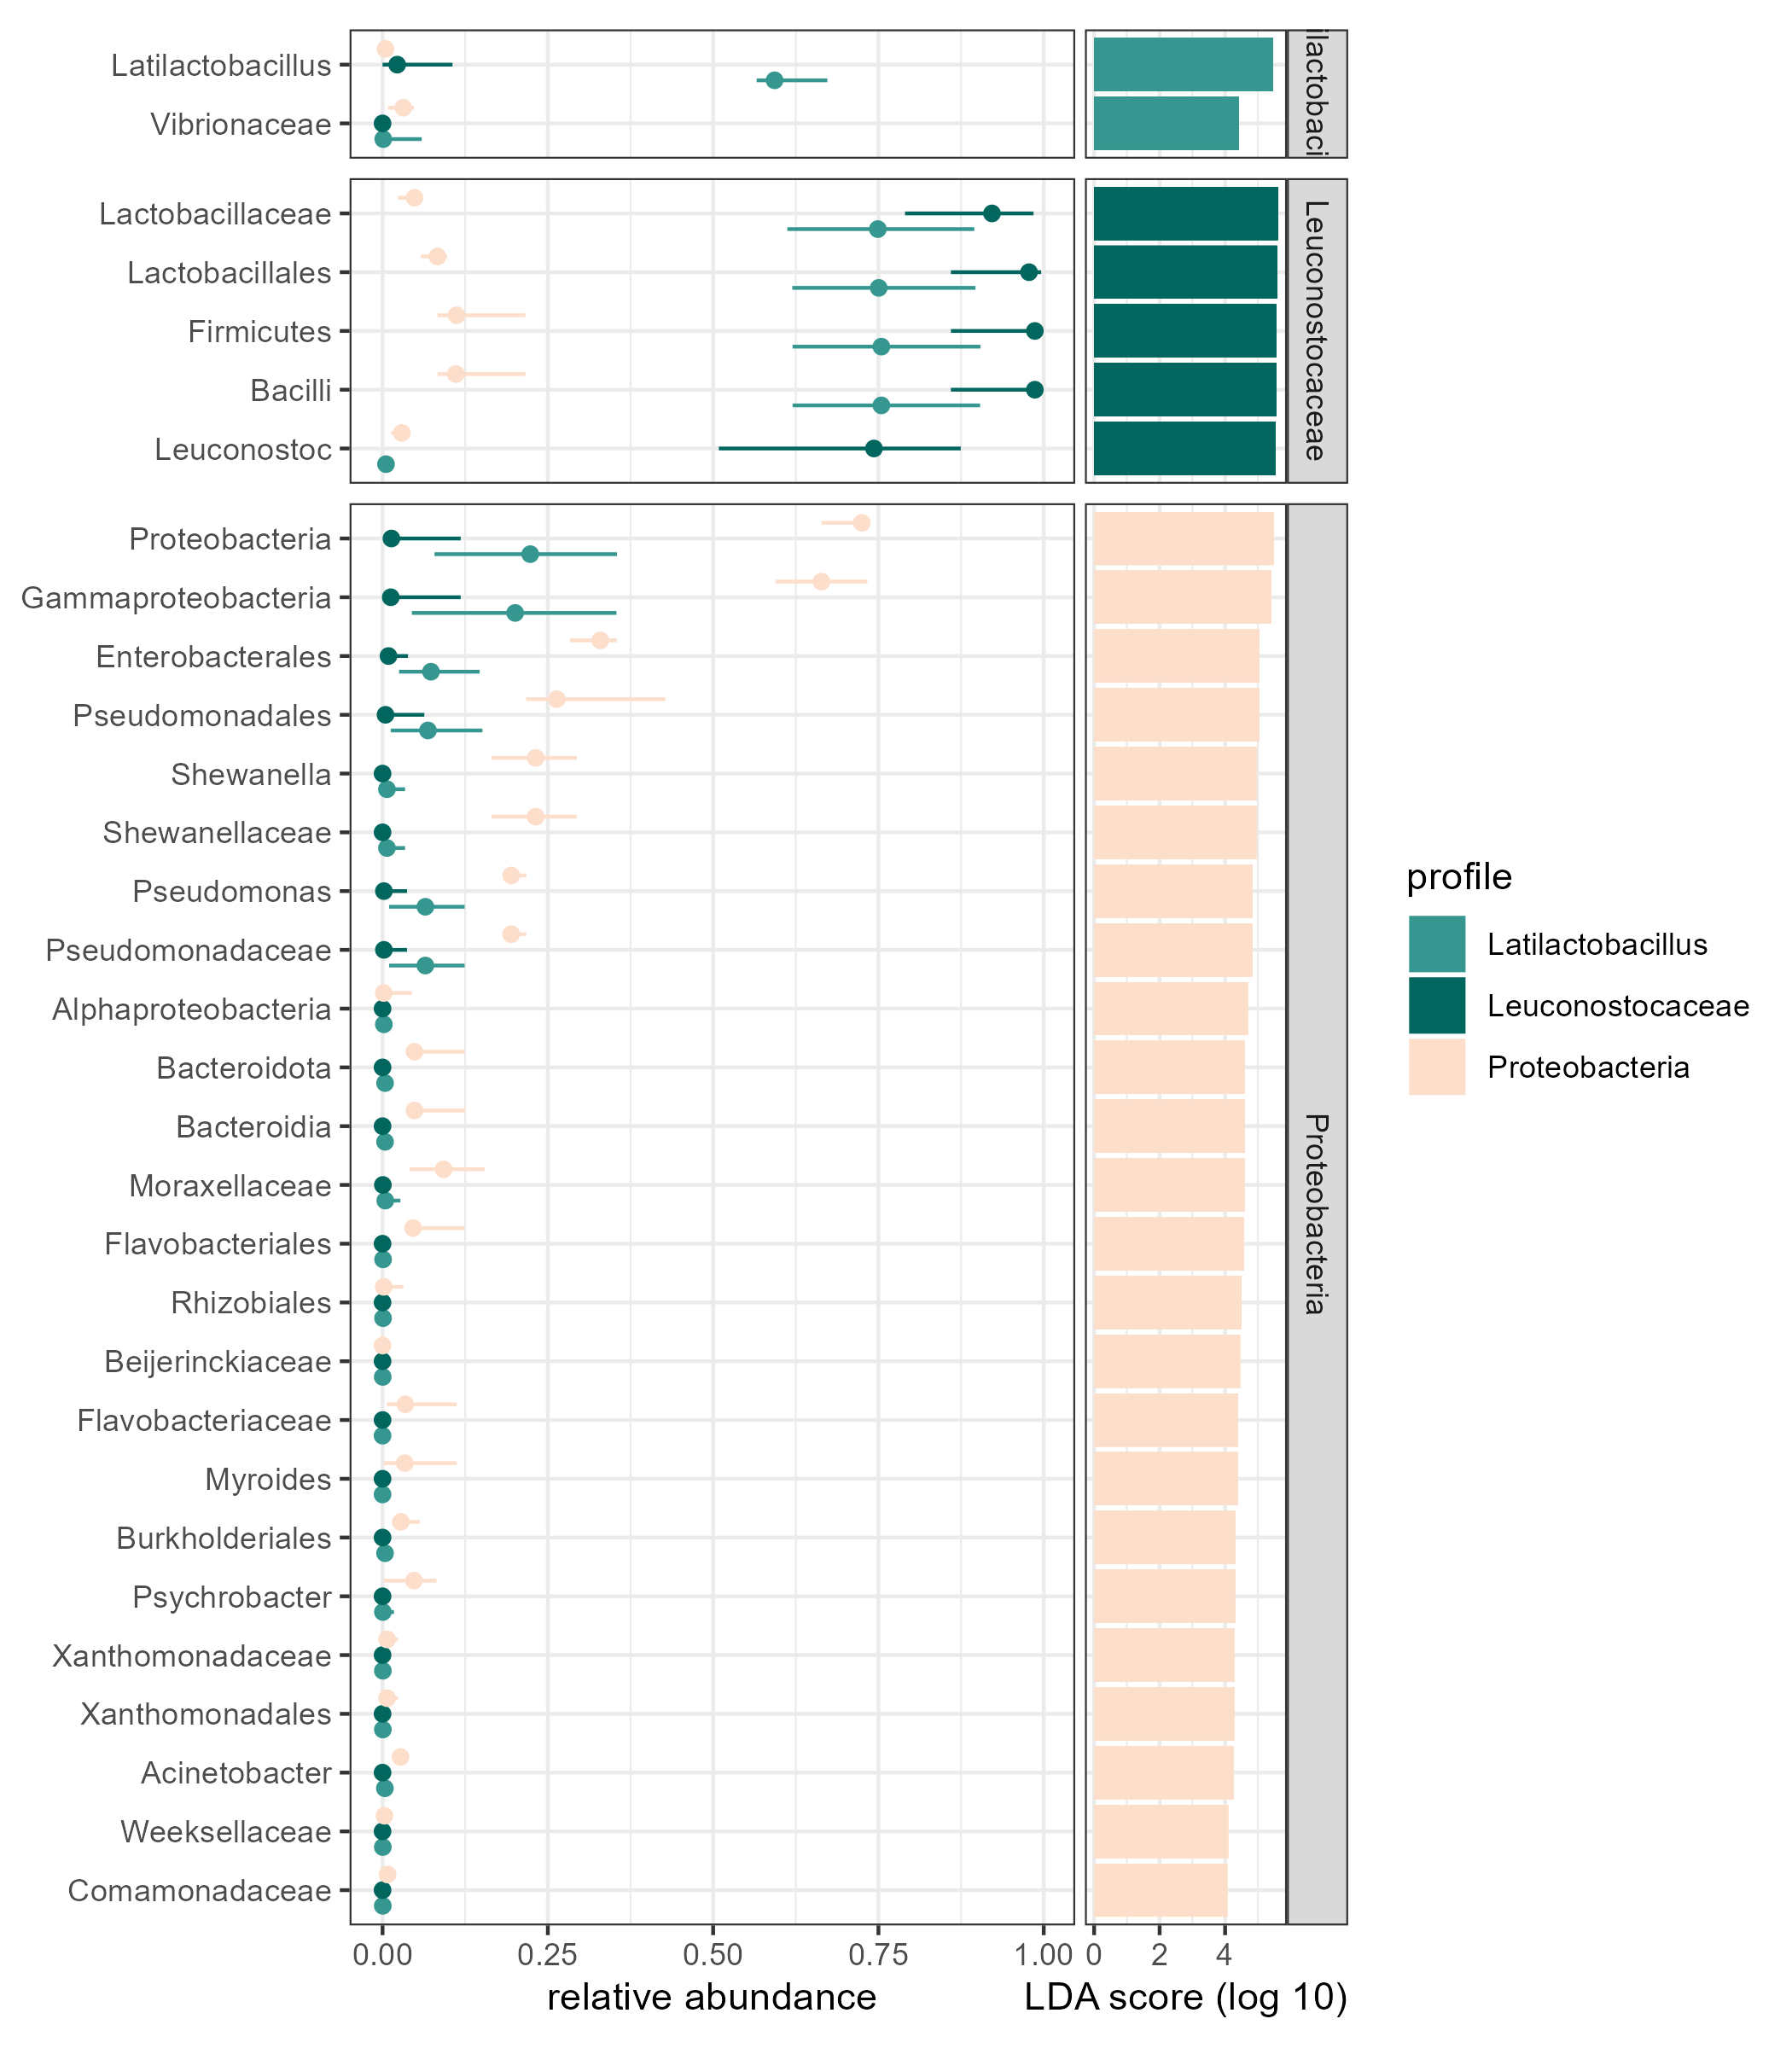
\includegraphics[width=1\linewidth]{lefsestatplot_profile} 

}

\caption{\label{figSM5} LEfSe per profile.  }\label{fig:figSM5}
\end{figure}

s 1 - alpha div group s 2 - NMDS s 3 - PERMANOVA res s 4 - LEfSE group s
5 - LEfSe profile

\newpage

\renewcommand\refname{References}
\bibliography{VeggieMeat.bib}


\end{document}
